\documentclass[MIRU,submit]{miru2026j}
\usepackage[dvipdfmx]{graphicx}
%\usepackage{latexsym}
\usepackage{booktabs}
\usepackage{colortbl}
\usepackage{amsmath}
\usepackage{amssymb}
\usepackage{amsthm}
\usepackage{mathtools}
\usepackage{pifont}
\usepackage{tabularx}
\usepackage{enumitem}
\usepackage{wrapfig}
\usepackage{multirow}
\usepackage{microtype}
\usepackage{float}
\usepackage{caption}
\usepackage{algorithm}
\usepackage{algorithmic}
\usepackage{cleveref}

% Okabe-Ito colors
\definecolor{PINK}{RGB}{230,159,0}
\definecolor{GREEN}{RGB}{0,158,115}
\definecolor{BLUE}{RGB}{0,114,178}
\definecolor{ORANGE}{RGB}{213,94,0}
\definecolor{PURPLE}{RGB}{204,121,167}
\definecolor{BLACK}{RGB}{0,0,0}
\definecolor{GRAY}{RGB}{99,99,99}
\definecolor{RED}{RGB}{255,0,0}

% Define mathematical symbols
\newcommand{\gM}{{\mathcal{M}}}
\newcommand{\gN}{{\mathcal{N}}}
\newcommand{\gT}{{\mathcal{T}}}
\newcommand{\R}{\mathbb{R}}
\newcommand{\dee}{{\mathrm{d}}}
\newcommand{\fst}[1]{$\mathbf{#1}$}
\newcommand{\snd}[1]{\underline{#1}}
\newcommand{\sss}[1]{{\scriptscriptstyle (#1)}}
\newcommand{\aster}{\makebox[0pt][l]{\smash{\textsuperscript{\tiny\!*}}}}
\newcommand{\asters}{\makebox[0pt][l]{\smash{\textsuperscript{\tiny\!*\!*}}}}

\begin{document}

\title{スコア関数のヤコビアンに基づく拡散モデルのリーマン計量}

\affiliate{Hokkaido}{北海道大学}
\affiliate{Cyber}{株式会社 サイバーエージェント AI Lab}

\author{齋藤 慎之介}{Shinnosuke SAITO}{Hokkaido}[saitou.shinnosuke.y0@elms.hokudai.ac.jp]
\author{松原 崇}{Takashi MATSUBARA}{Hokkaido, Cyber}[matsubara@ist.hokudai.ac.jp]

\maketitle

% \begin{figure}[t]
%    \centering
%    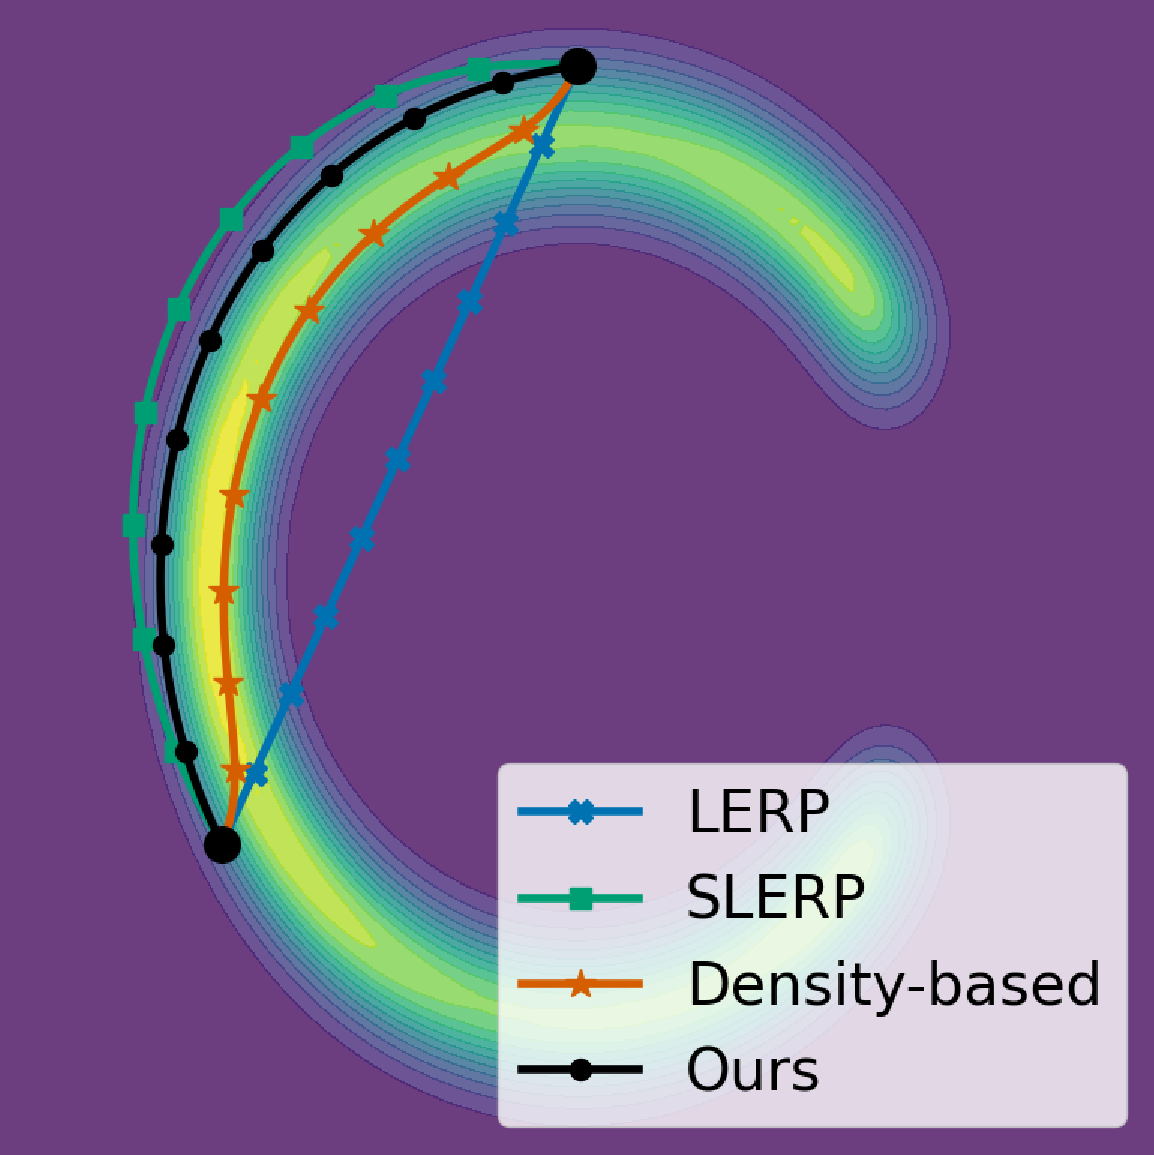
\includegraphics[width=0.3\textwidth]{assets/concept/geodesic.pdf}
%    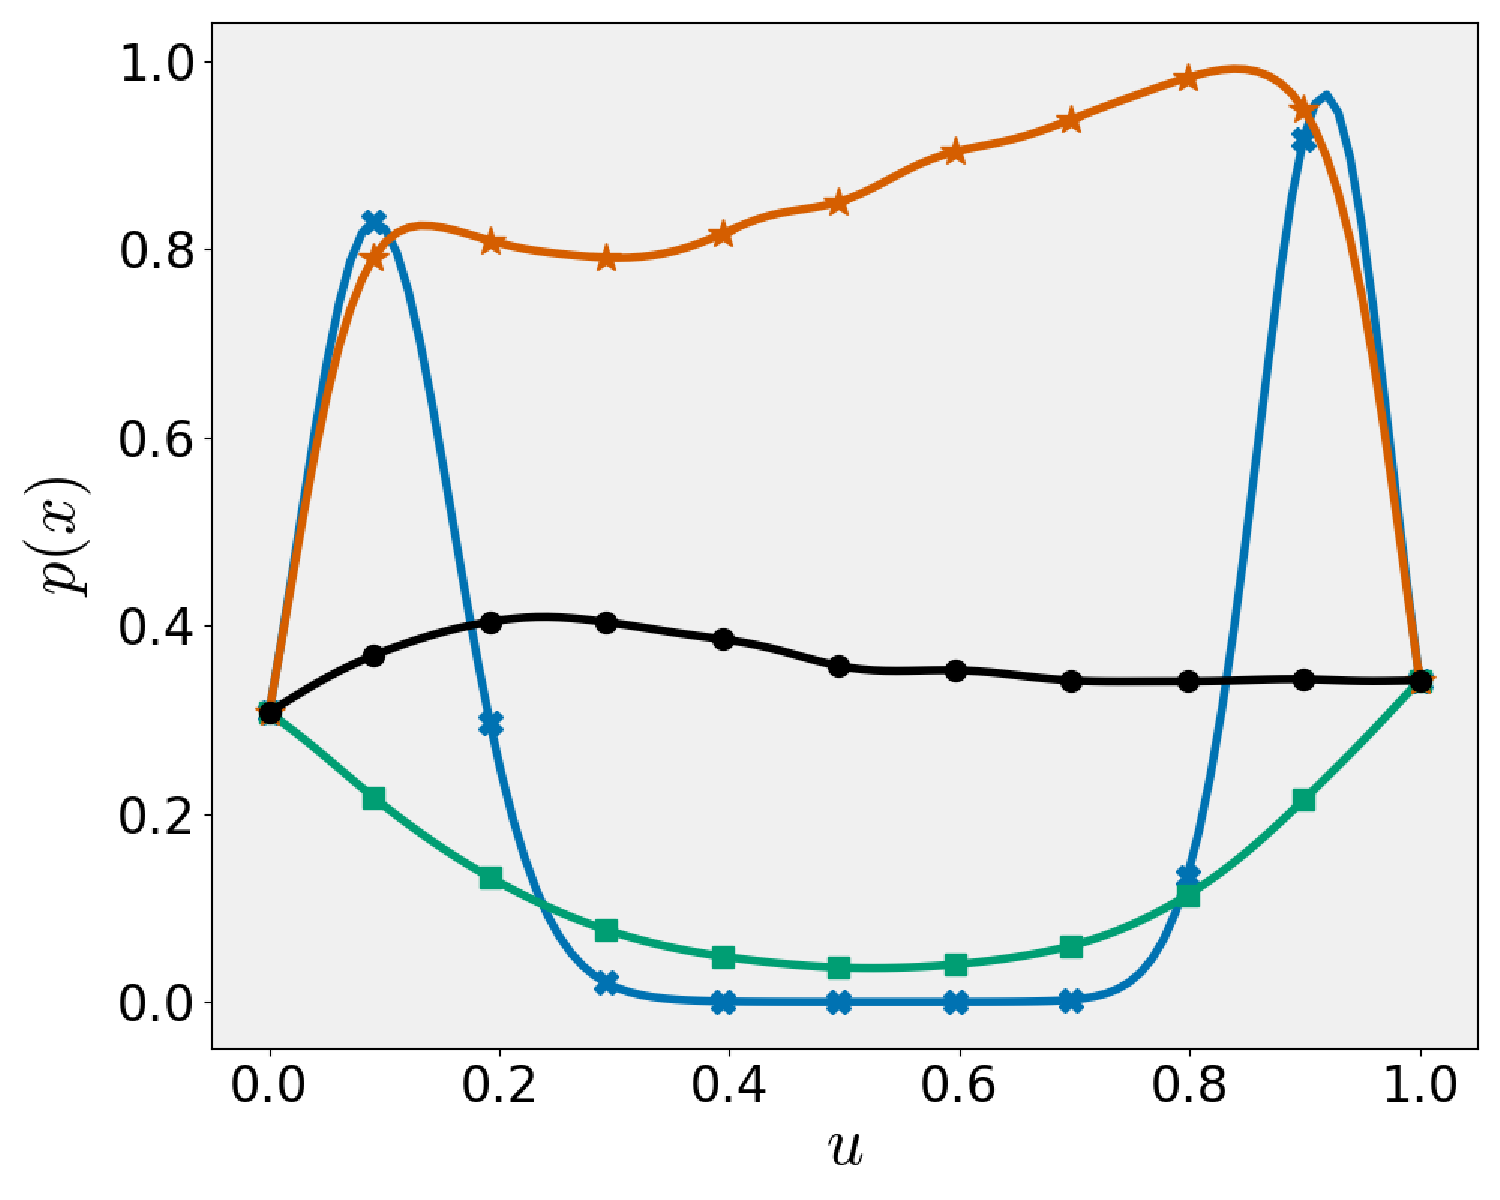
\includegraphics[width=0.4\textwidth]{assets/concept/density.pdf}
%    \caption{補間パスの比較．（左）C字形分布上の補間経路．（右）各手法の確率密度の遷移．}
%    \label{fig:illust}
% \end{figure}

% \begin{figure}[t]
%    \centering
%    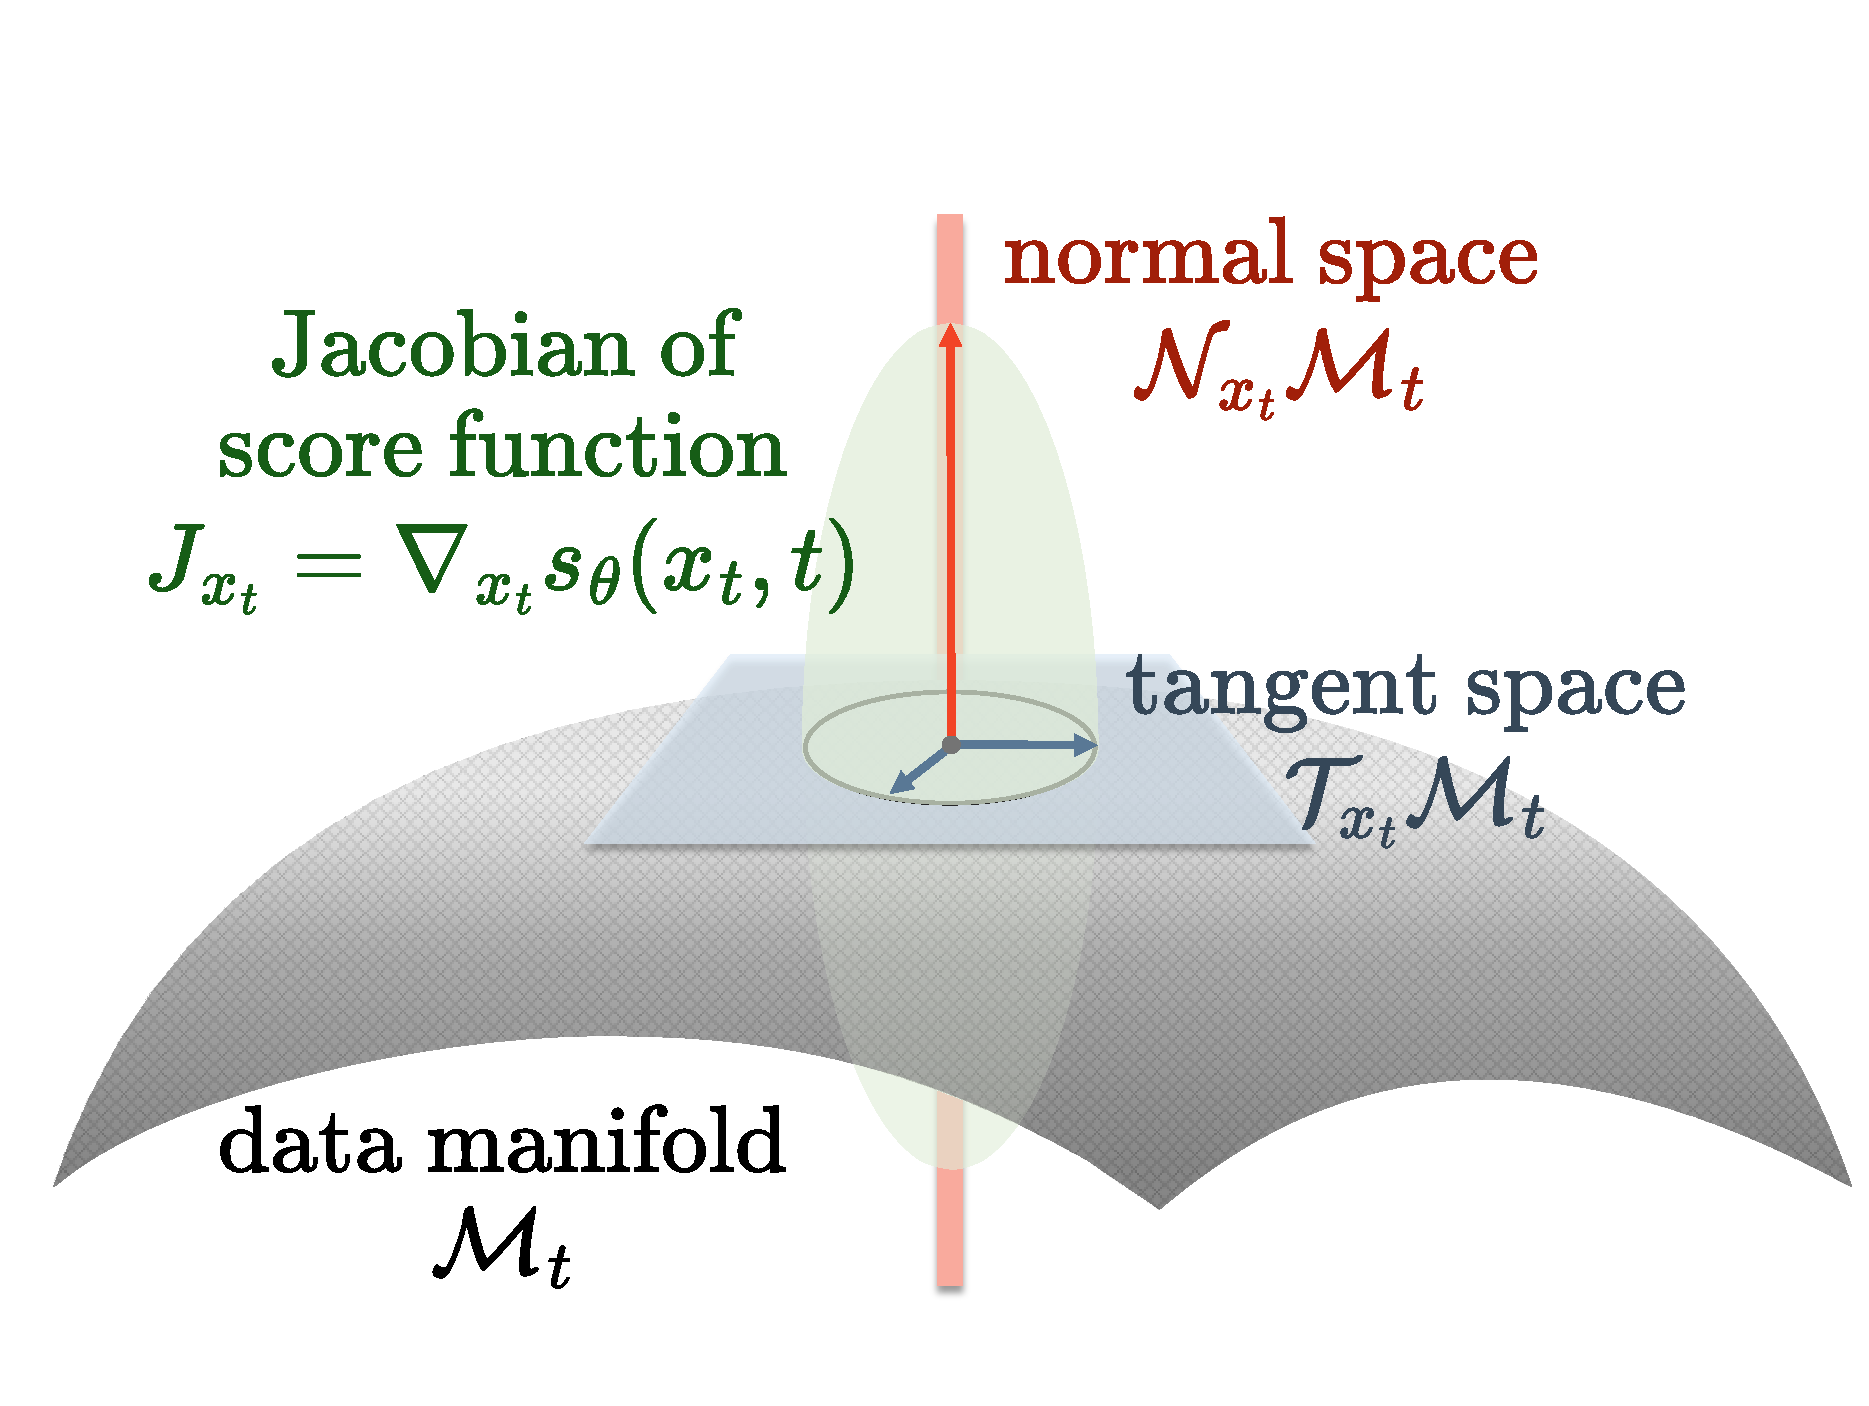
\includegraphics[width=0.4\textwidth]{assets/concept/metric.pdf}
%    \caption{概念図．スコア関数のヤコビアン $J_{x_t}$ のスペクトル構造が接線空間 $\mathcal{T}_{x_t}\mathcal{M}_t$ と法線空間 $\mathcal{N}_{x_t}\mathcal{M}_t$ を分離する．}
%    \label{fig:concept}
% \end{figure}

% \begin{figure}[t]
%     \centering
%     \footnotesize

%     % Top row: (a) and (b)
%     \setlength{\tabcolsep}{2pt}
%     \begin{tabular}{cc}
%         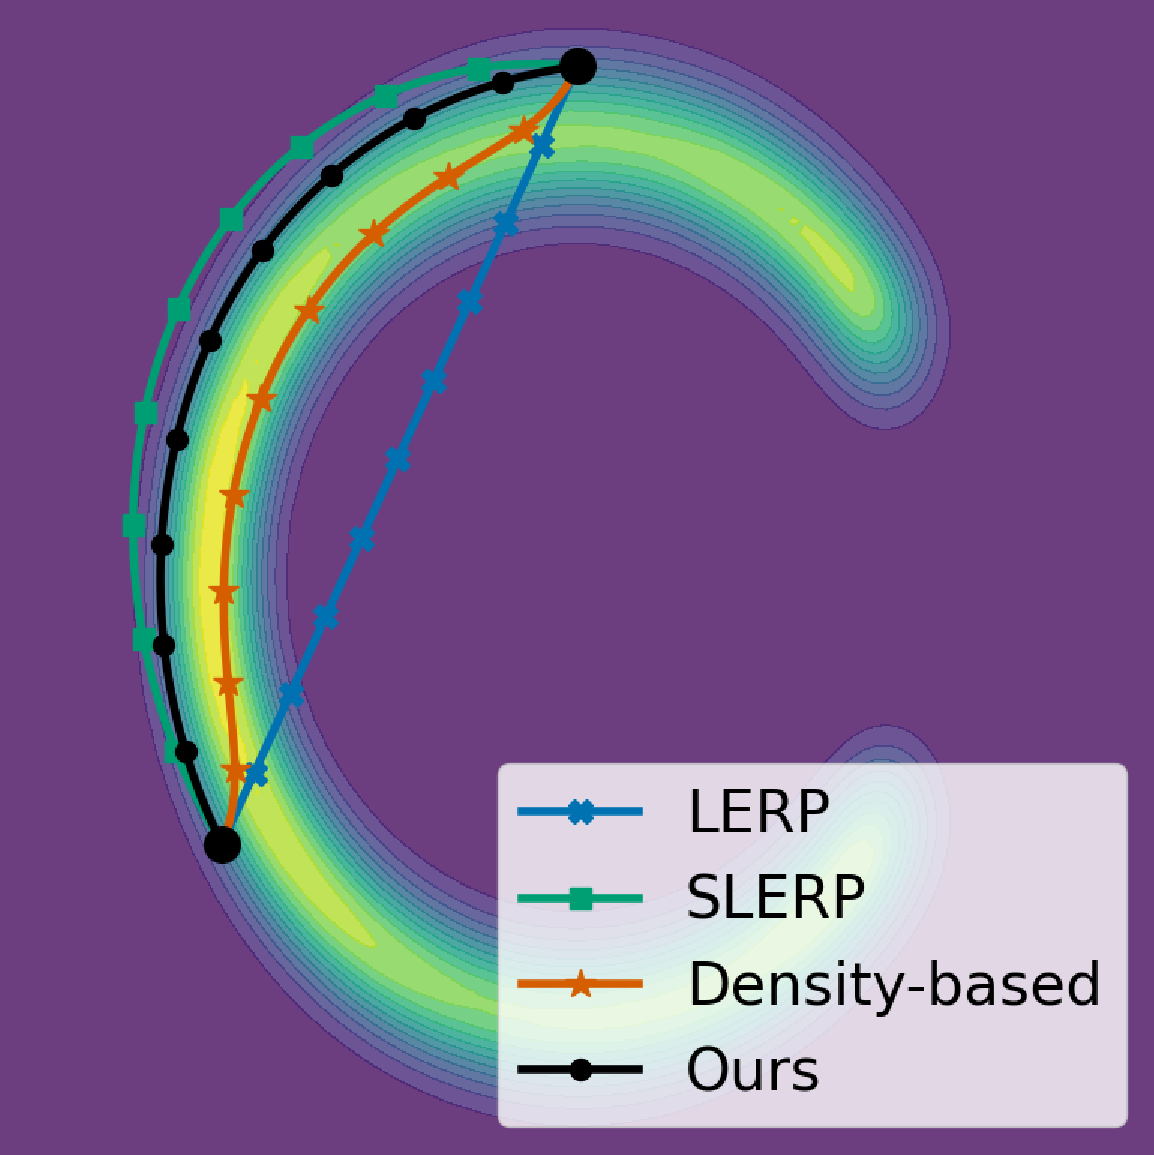
\includegraphics[width=3.5cm]{assets/concept/geodesic.pdf} &
%         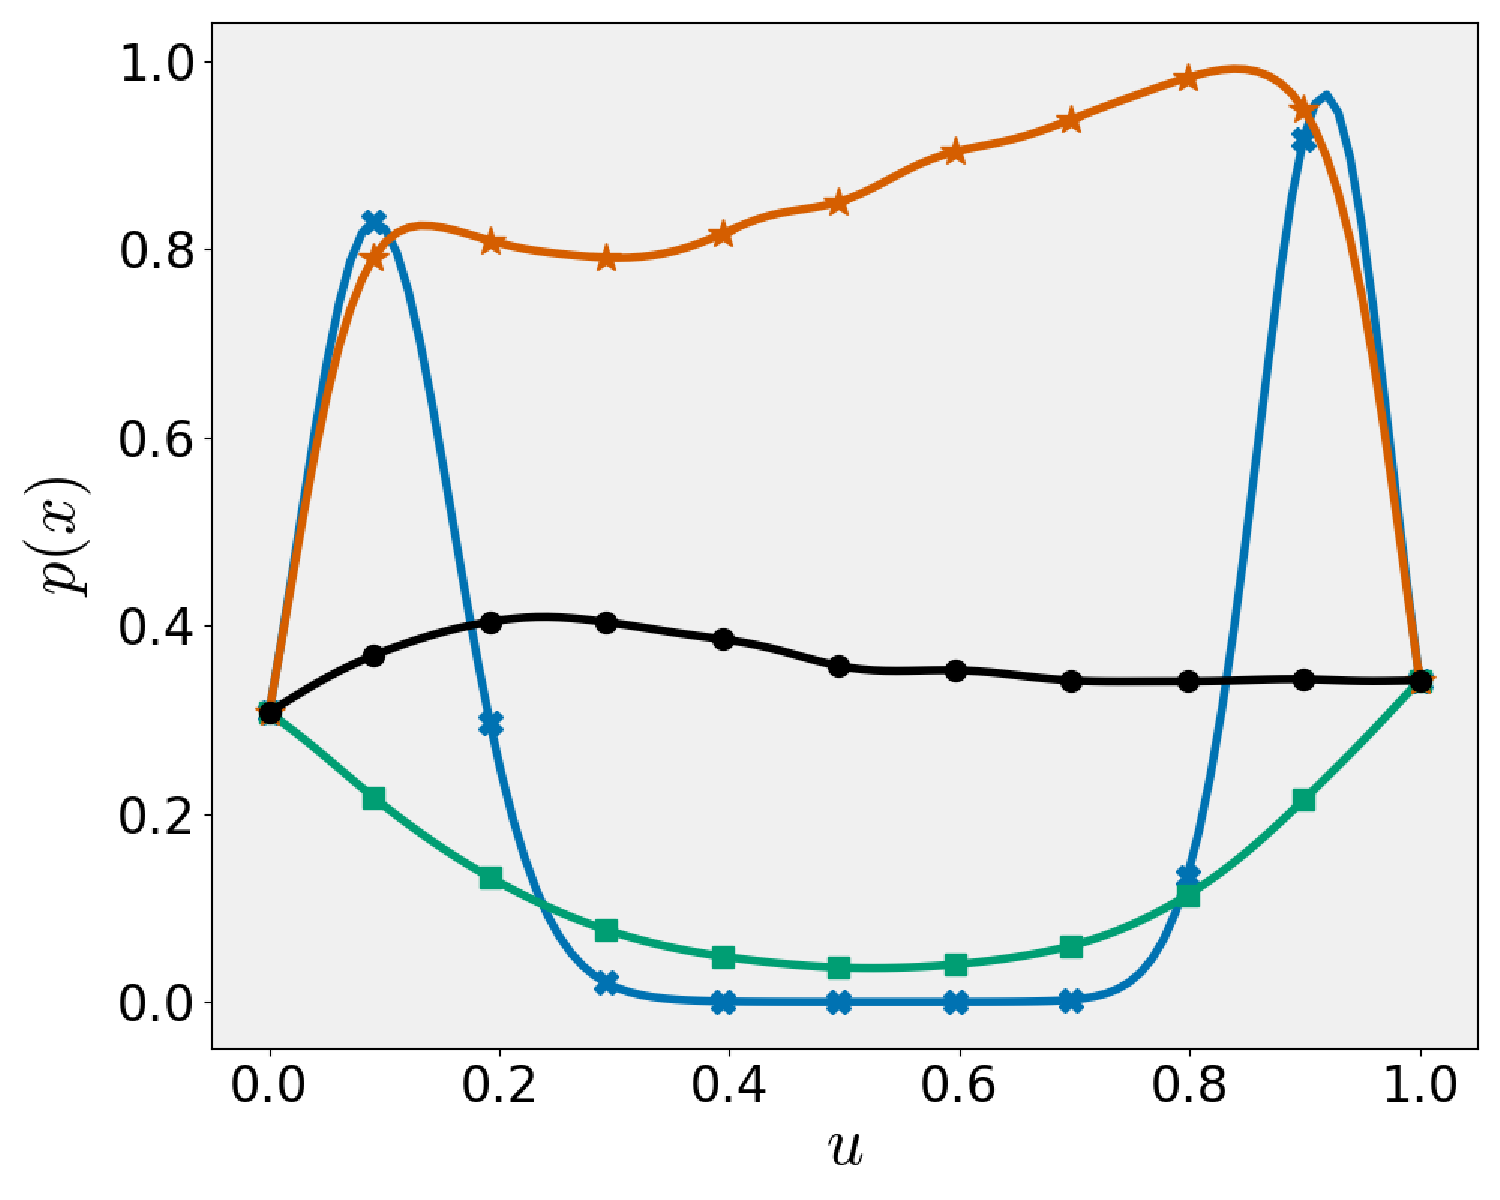
\includegraphics[width=4.5cm]{assets/concept/density.pdf} \\
%         (a) & (b)
%     \end{tabular}
%     \vspace{3pt}
%     \begin{tabular}{c}
%         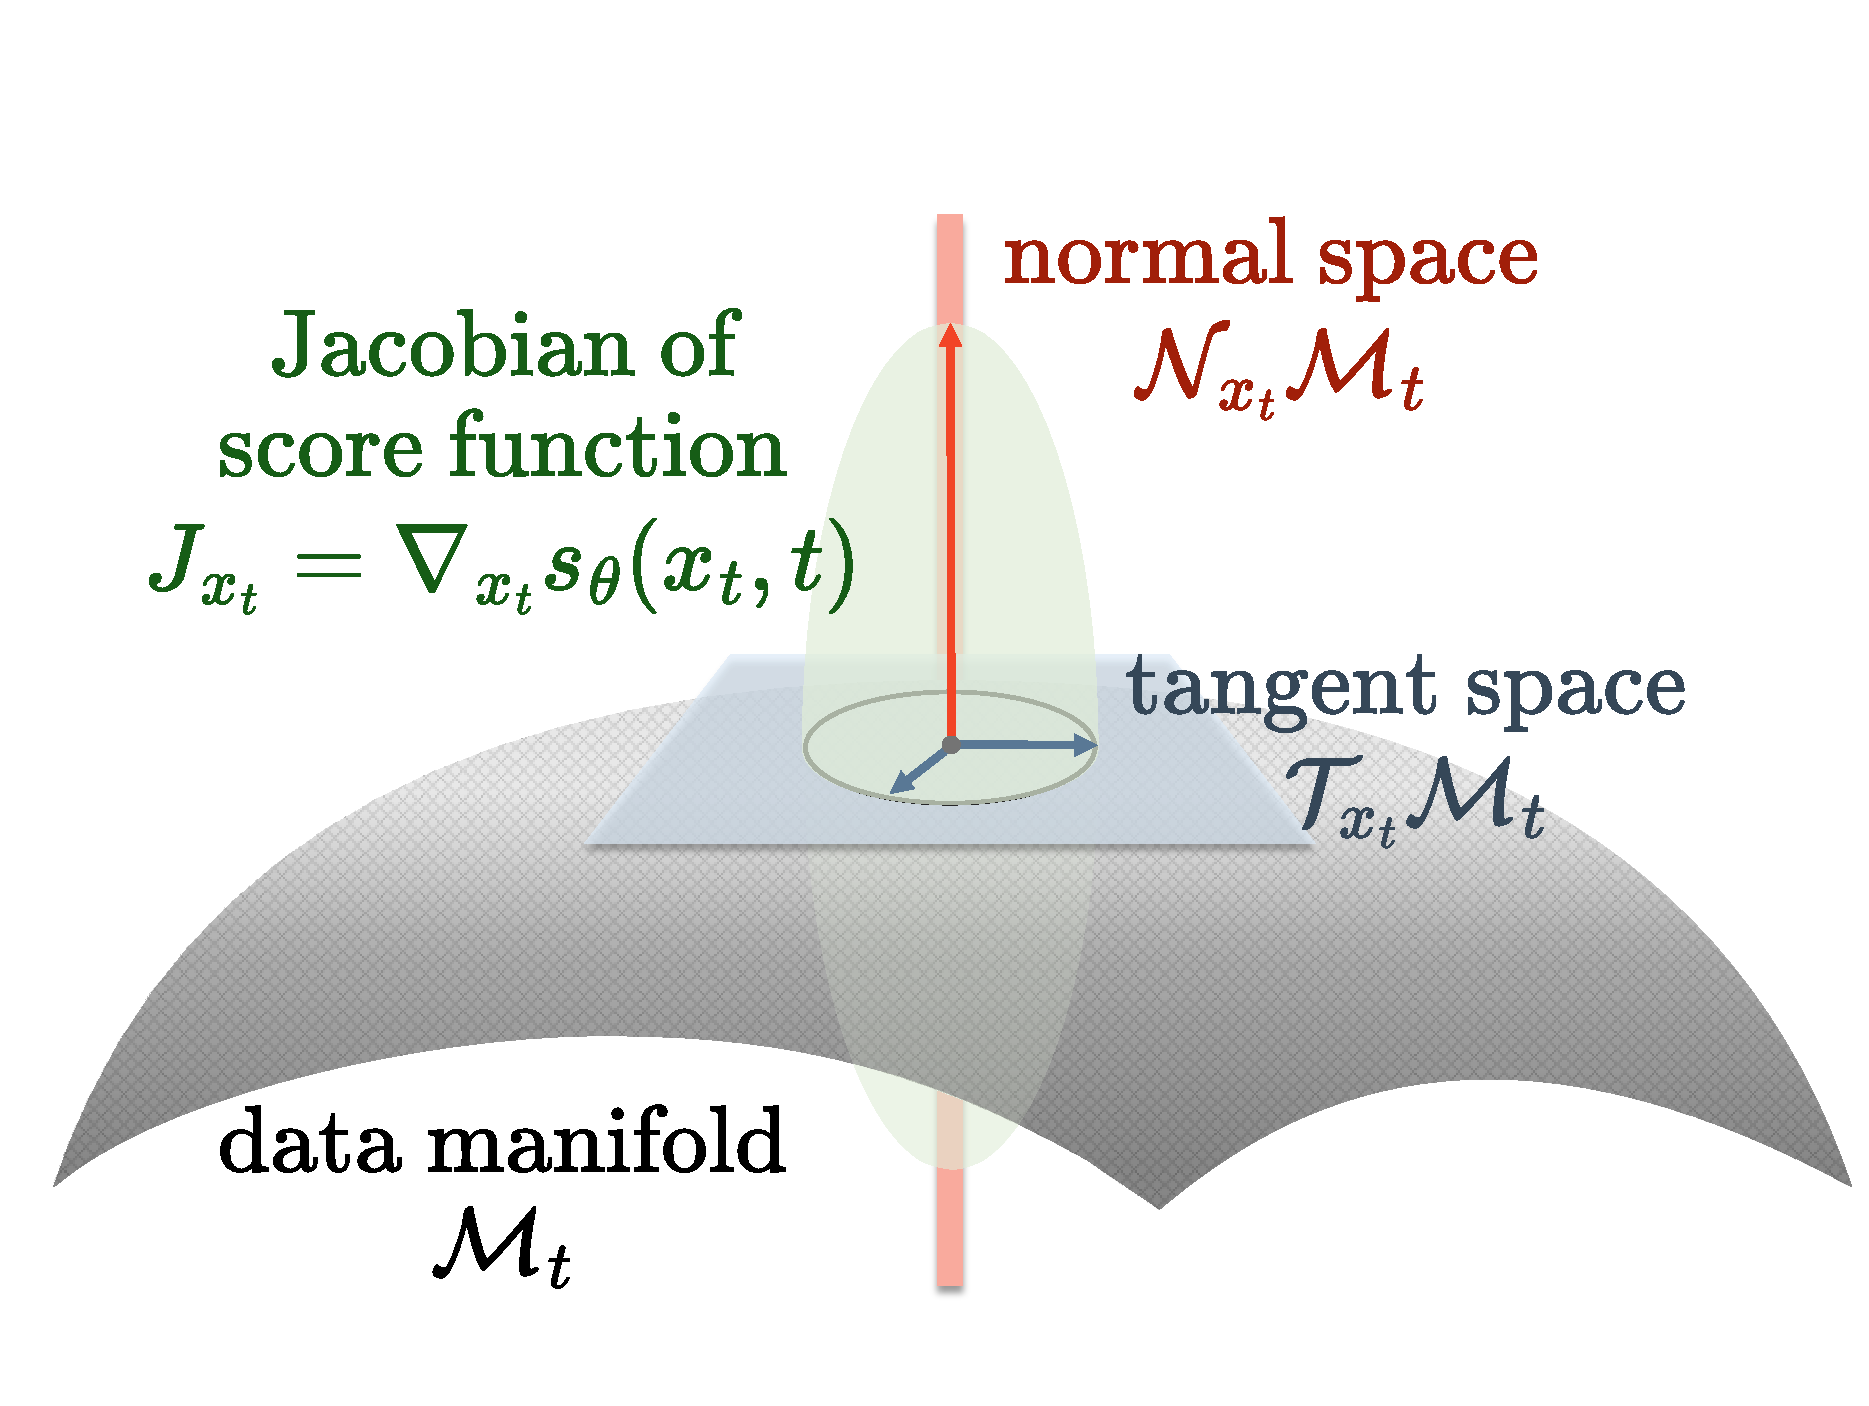
\includegraphics[width=0.4\textwidth]{assets/concept/metric.pdf} \\
%         (c)
%     \end{tabular}

%     \caption{
%         \textbf{A conceptual comparison of interpolation.}
%         (a) Interpolation paths on a C-shaped distribution.
%         (b) A plot of the probability density transitions for their corresponding interpolation paths.
%         (c) Examples of image interpolation on Animal Faces-HQ \cite{Choi2022b}.
%     }
%     \label{fig:concept}
% \end{figure}

\begin{figure*}[!ht]
    \centering
    \footnotesize
    \setlength{\tabcolsep}{2pt}
    \begin{tabular}{ccc}
        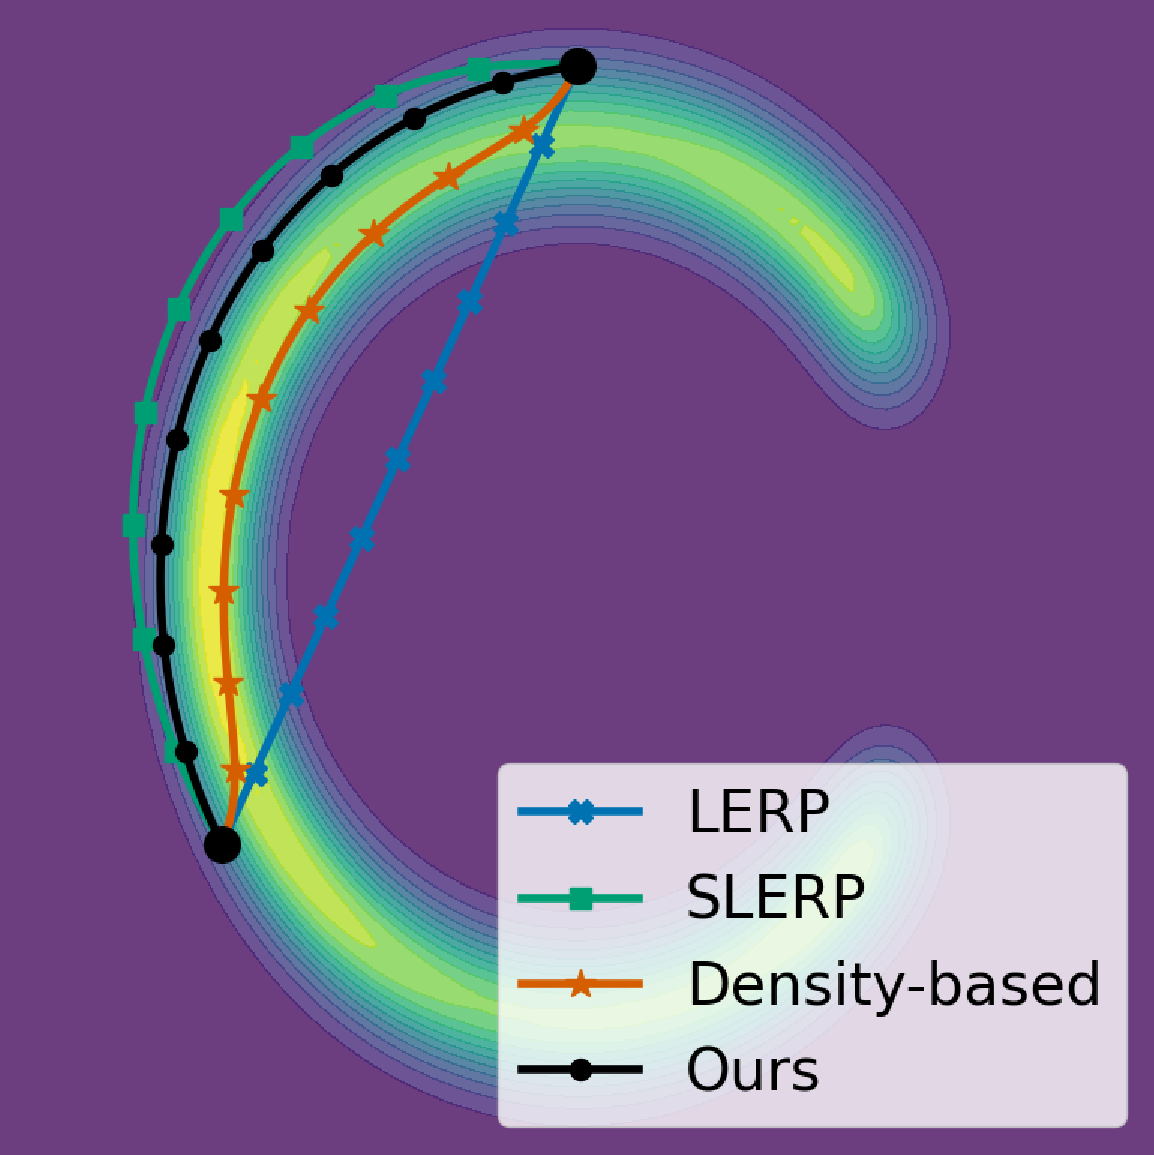
\includegraphics[width=0.25\textwidth]{assets/concept/geodesic.pdf} &
        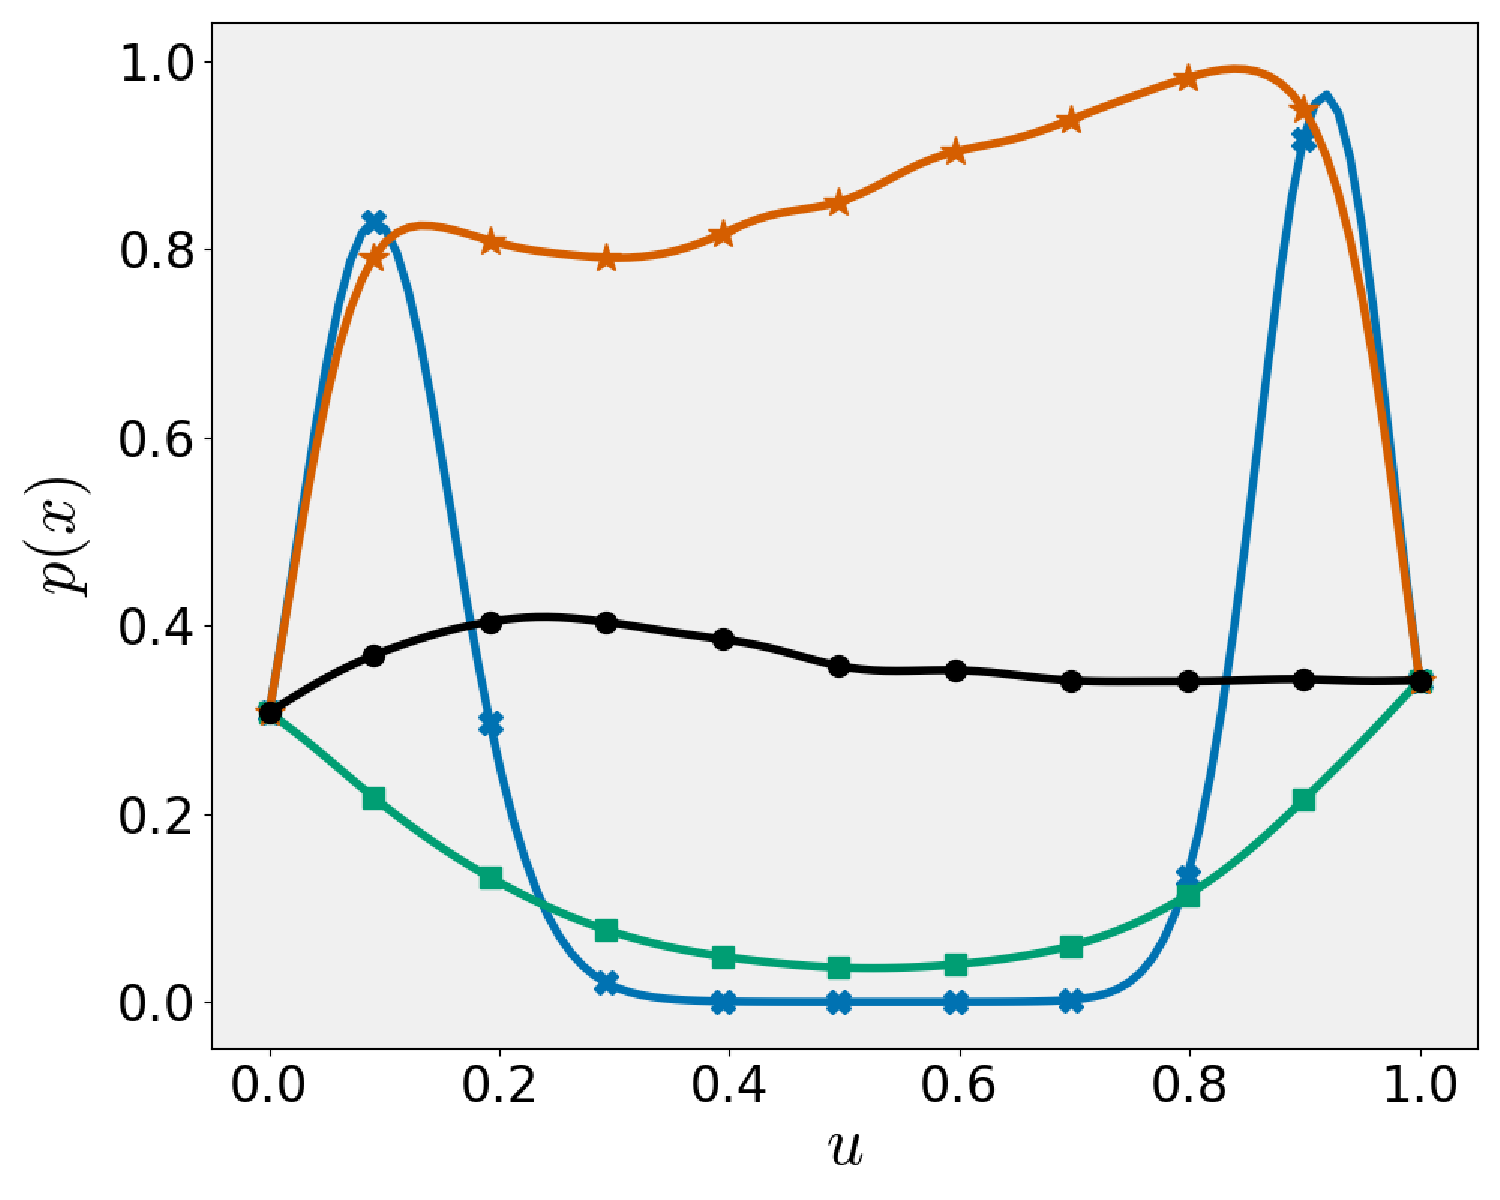
\includegraphics[width=0.32\textwidth]{assets/concept/density.pdf} &
        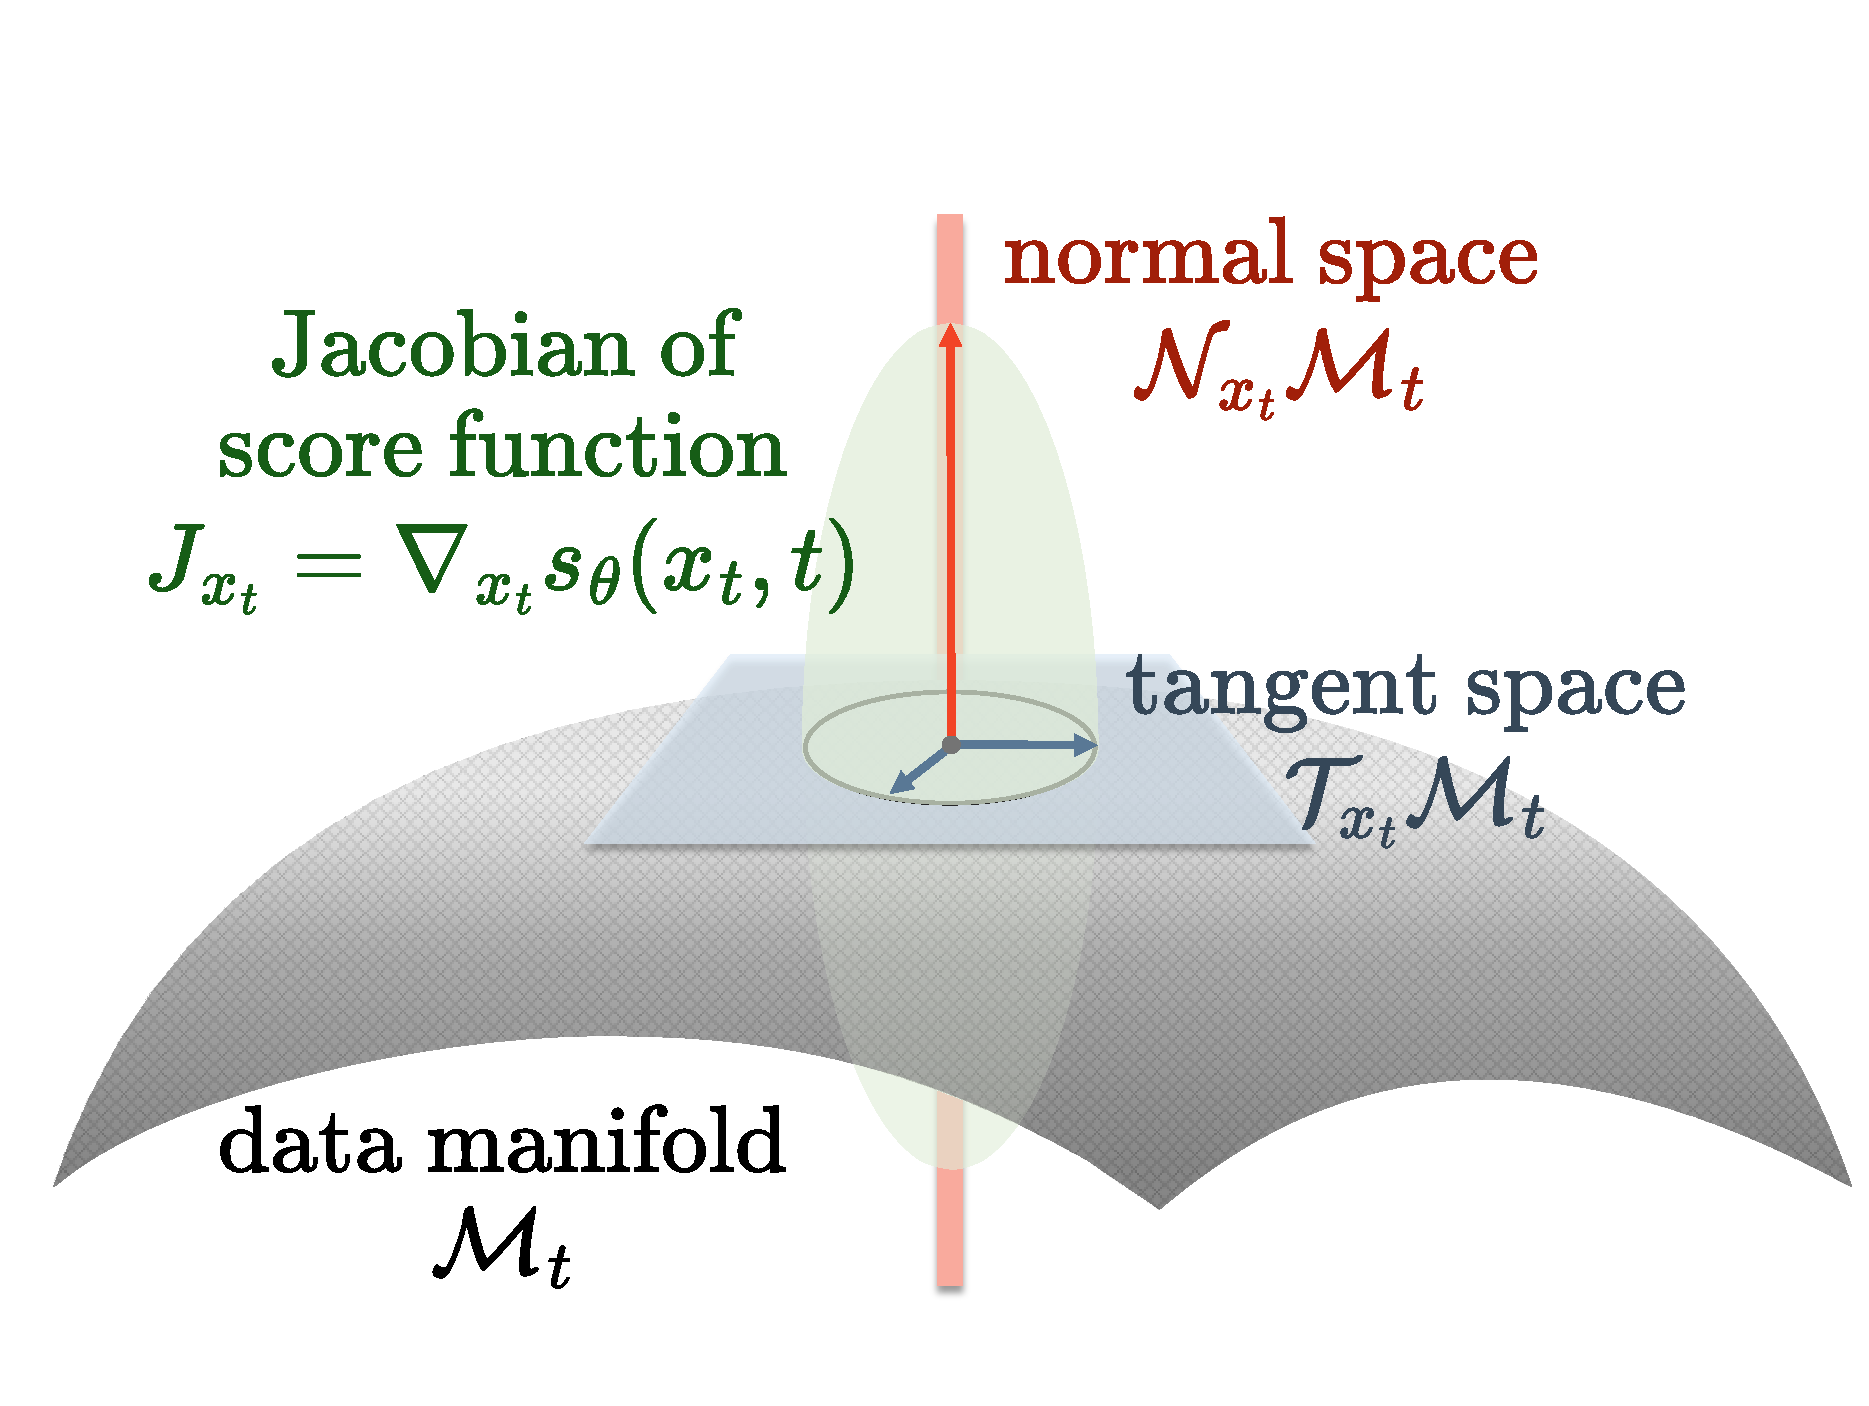
\includegraphics[width=0.4\textwidth]{assets/concept/metric.pdf} \\
        (a) & (b) & (c)
    \end{tabular}
    \caption{
        \textbf{概念図.}
        (a) C字形分布上の補間経路．
        (b) 各手法の確率密度の遷移．
        (c) スコア関数のヤコビアン $J_{x_t}$ のスペクトル構造が接空間 $\mathcal{T}_{x_t}\mathcal{M}_t$ と法空間 $\mathcal{N}_{x_t}\mathcal{M}_t$ を分離する．
    }
    \label{fig:concept_wide}
\end{figure*}

\section*{概要}
拡散モデルは明示的で扱いやすい低次元潜在空間を持たないため，データ多様体を考慮した操作が困難である．
本稿では，スコア関数のヤコビアンのスペクトル構造が多様体の接線・法線方向を分離するという知見に基づき，経路が接線方向に沿うよう促す，ノイズ空間上の学習不要なリーマン計量を提案する．
実験により，本計量が多様体からの逸脱を抑え，測地線による自然な補間と，分類器なしガイダンスでの生成品質の向上を確認した．

\section{はじめに}

拡散モデルは，高品質かつ多様なデータを生成できる深層生成モデル（DGM）の一種である~\cite{Ho2020,Song2021a,Rombach2022}．
DGM を理解・改善するための重要な視点として多様体仮説がある．
これは，実世界のデータ（例：画像）が高次元空間に埋め込まれた低次元多様体の周囲に集中しているという仮定である~\cite{Bengio2012,Fefferman2016}．
この仮定のもとでは，DGMはデータ分布だけでなく，その背後にある多様体構造を暗黙的または明示的に学習していると解釈される~\cite{Loaiza-ganem2024}．

VAE~\cite{Kingma2014}やGAN~\cite{Goodfellow2014}は，データ多様体を陽にパラメータ化する低次元潜在空間を持つ．
そのため，デコーダを通じた引き戻しによりリーマン計量を定義でき~\cite{Gruffaz2025}，測地線に沿った潜在空間の移動がデータの幾何構造に忠実な補間を与える~\cite{Shao2017,Arvanitidis2018,Chen2018,Arvanitidis2021}．
一方，拡散モデルはそのような低次元潜在空間を持たず，ノイズ空間はデータ空間と同次元であるため，引き戻し計量の定義は非自明である．

先行研究では，ノイズサンプルの密度や多様体への方向に基づくリーマン計量が提案されている~\cite{Yu2025,Azeglio2025}（\cref{fig:illust}）．
しかし，こうした計量では測地線が高密度領域に過度に引き寄せられ，生成結果が過度に平滑化されることが指摘されている~\cite{Karczewski2025a}．
これは，密度や方向がサンプルの集中する位置を捉える一方で，多様体が環境空間内でどう広がっているかという配向の情報を含まないためである．
では，密度ではなく多様体の幾何構造そのものを反映する計量は定義できるだろうか．

本稿では，スコア関数のヤコビアンが多様体の配向をすでに符号化しているという事実に着目する：そのスペクトル構造はデータ多様体の接線方向と法線方向を分離する~\cite{Stanczuk2024,Ventura2025}（\cref{fig:concept}）．
この性質を利用し，スコア関数によるユークリッド計量の引き戻しとしてノイズ空間上のリーマン計量を定義する．
提案計量は法線方向の移動に高いコストを，接線方向には低いコストを課すため，経路を多様体に沿う方向へ誘導する．
さらに，事前学習済みスコア関数のヤコビアンのみから構成でき，追加の学習やアーキテクチャ変更を要しない．

本稿の貢献は，この計量の定義と，それに基づくノイズ空間の接線・法線分解にある．
提案計量の妥当性を以下の二つの観点から検証する．
\textbf{(i)~測地線補間による大域的幾何の検証}（\cref{sec:synthetic,sec:image_interp,sec:video_interp}）：
提案計量のもとでの測地線は多様体に沿って推移し，知覚的に自然な遷移をもたらす．
合成データ，画像，動画フレームの各データセットでこれを確認する．
\textbf{(ii)~ガイダンス補正による局所的幾何の検証}（\cref{sec:guidance}）：
提案計量の接線・法線分解を用いて，Classifier-Free Guidance（CFG）~\cite{Ho2021}によるサンプルの多様体からの逸脱を抑制する．
この補正はCLIPスコアを維持しつつFIDを一貫して改善し，蒸留モデルにも追加コストなく適用できる．

\section{関連研究}

\subsection{深層生成モデルのリーマン幾何}
VAE や GAN では，データ多様体をパラメータ化している潜在空間上で，線形操作に基づく意味属性の編集が広く行われてきた~\cite{Goetschalckx2019,Harkonen2020,Shen2020}．
一方で，実データ分布の偏りに伴う非線形な変動を考慮した手法も提案されているが~\cite{Jahanian2020,Aoshima2023}，これを体系的に扱う枠組みとして，潜在空間へのリーマン計量の導入が研究されている~\cite{Gruffaz2025}．
計量の構成法は大きく二つに分かれ，追加のネットワークで計量を学習する手法~\cite{Yang2018,Arvanitidis2022}と，事前学習済みデコーダを通じた引き戻し計量を用いる学習不要な手法~\cite{Shao2017,Chen2018,Arvanitidis2018,Arvanitidis2021}が知られている．
前者は元の多様体構造を上書きする恐れがあるのに対し，後者はモデルが学習した幾何を直接利用できる．
本研究は後者のアプローチを，ノイズ空間が低次元でない拡散モデルへと拡張する．

\subsection{拡散モデルにおけるデータ多様体}
拡散モデルは，スコア関数 $s_\theta(x_t, t)$ を通じて時刻 $t=T$ から $t=0$ へ段階的にノイズ除去を行い，データ分布を学習する~\cite{Ho2020,Song2021a,Song2021b}．
$t>0$ におけるノイズサンプルの空間はしばしばノイズ空間と呼ばれる．
拡散モデルはこの除去過程を通じてデータ多様体を暗黙的に学習することが知られている~\cite{Pidstrigach2022,Tang2024}．
特に重要な知見として，スコア関数のヤコビアンはデータ多様体の余次元に対応するランク欠損，あるいは急峻なスペクトルギャップを示し，これが多様体の法線方向と接線方向を分離することが報告されている~\cite{Stanczuk2024,Ventura2025}．
本研究では，密度に依拠せず，このスペクトル的特性に基づいてノイズ空間上のリーマン計量を定義する．

\subsection{拡散モデルにおける補間}
ノイズ空間における補間手法は大きく四つに分類できる．
(i)~\textbf{閉形式手法}：LERP~\cite{Ho2020} はユークリッド空間として扱うがノルムが小さくなる，SLERP~\cite{Shoemake1985,Song2021a} は超球面上でノルムを保存する~\cite{Samuel2023,Zheng2024}．
(ii)~\textbf{代替潜在空間手法}：拡散ネットワークの中間層を利用するが~\cite{Kwon2023,Park2023a}，スキップ接続により自己完結的な表現としての能力に限界がある．
(iii)~\textbf{追加学習依存手法}：補間用の追加ネットワークや構造変更を必要とする~\cite{Kaiwen2023,Guo2024,Hahm2024,Kim2025}．
(iv)~\textbf{リーマン計量ベース手法}：追加学習なしにノイズ空間の幾何を定義する~\cite{Yu2025,Azeglio2025}．これらはノイズサンプルの密度に基づく計量を用いるため測地線が高密度領域へ引き寄せられ，過平滑化された補間をもたらす恐れがある~\cite{Karczewski2025a}．
本手法は (iv) に属するが，密度ではなくスコアヤコビアンのスペクトル構造を利用することで，測地線をデータ多様体の接線方向に保つ点で根本的に異なる．

\subsection{条件付き生成におけるガイダンス手法}
拡散モデルで条件付き生成するために用いる分類器なしガイダンス（CFG）~\cite{Ho2021} は，テキスト条件への忠実度を高める一方，学習済みのデータ多様体を歪め，視覚的に不自然な生成結果をもたらすことが知られている．
この問題を緩和するために，CFG++~\cite{Chung2025} は再ノイズ化ステップに無条件スコアを用い，TCFG~\cite{Kwon2025} は SVD により無条件スコアを条件付きスコアと共有する部分空間へ射影する．
これらの手法はデータ多様体の存在に動機付けられているが，その幾何を形式的に定義・特徴付けるものではなく，補正はヒューリスティックにとどまる．
本手法はこのような幾何的特性付けを提供し，ガイダンス項を接線成分と法線成分に分解して後者を抑制するという幾何学的に根拠のある補正を可能にする．

\section{提案手法}

\subsection{提案リーマン計量}

\subsubsection{定義}
スコア関数を通じて，データ多様体の局所幾何を捉えるノイズ空間上のリーマン計量を定義する．
$x_t \in \mathbb{R}^D$ をノイズ空間中の点，$v, w \in T_{x_t}\mathbb{R}^D$ を接ベクトル，$s_\theta(x_t, t)$ を事前学習済み拡散モデルのスコア関数とする．
時刻 $t$ における提案計量を以下のように定義する：
\begin{equation}
    \textstyle
    \label{eq:jacobian_metric}
    g_{x_t}(v, w) \coloneqq \langle J_{x_t} v,\, J_{x_t} w \rangle = v^\top G_{x_t}\, w, 
\end{equation}
ここで $J_{x_t} = \nabla_{x_t} s_\theta(x_t, t)$ はスコア関数のヤコビアン，$G_{x_t} = J_{x_t}^\top J_{x_t}$ は計量の行列表現である．
この計量はスコア空間 $\mathbb{R}^D$ 上のユークリッド計量 $I$ のスコア関数 $s_\theta$ を通じた引き戻し計量 $s_\theta^* I$ である．

\subsubsection{解釈．}
Stanczuk ら~\cite{Stanczuk2024} はスコア関数 $s_\theta(x_t, t)$ がデータ多様体 $\mathcal{M}_t$ に対して直交する方向を向くことを示した．
Ventura ら~\cite{Ventura2025} はさらにヤコビアン $J_{x_t}$ のスペクトルギャップがデータ多様体の内在次元を反映することを明らかにした．
直感的には，$J_{x_t}$ は接線方向へは小さく，法線方向へは大きく作用する（\cref{fig:concept}）．

より正確には，$J_{x_t}$ の小さい特異値に対応する右特異ベクトルが張る $d$ 次元部分空間を接線空間 $\mathcal{T}_{x_t}\mathcal{M}_t$，大きい特異値に対応するものが張る空間を法線空間 $\mathcal{N}_{x_t}\mathcal{M}_t$ と定義すると，$T_{x_t}\mathbb{R}^D = \mathcal{T}_{x_t}\mathcal{M}_t \oplus \mathcal{N}_{x_t}\mathcal{M}_t$ が成り立つ．

% \begin{proposition}
%     \label{thm:equivalence}
%     固定されたユークリッドノルムを持つ接ベクトル $v$ のうち，計量ノルム $g_{x_t}(v,v) = \|J_{x_t} v\|_2^2$ が最小となるものは，データ多様体 $\mathcal{M}_t$ の接線空間 $\mathcal{T}_{x_t}\mathcal{M}_t$ に属する．
% \end{proposition}

したがって，提案計量はデータ多様体上またはその接線方向に沿って推移する経路に短い長さを割り当てる．

\subsubsection{測地線}
測地線はエネルギー汎関数 $E[\gamma]$ を最小化する最短経路である．
$u \in [0,1]$ で曲線 $\gamma$ をパラメータ化すると，提案計量のエネルギー汎関数は
\begin{equation}
    \textstyle
    \label{eq:energy_jacobian_revisit}
    \begin{aligned}
        E[\gamma]
        &= \frac{1}{2}\int_0^1 \|J_{\gamma(u)} \gamma'(u)\|_2^2\, \mathrm{d}u \\
        &= \frac{1}{2}\int_0^1 \left\|\frac{\partial}{\partial u} s_\theta(\gamma(u), t)\right\|_2^2 \mathrm{d}u.
    \end{aligned}
\end{equation}
右辺の最後の表現（連鎖律による）は，測地線がスコア関数 $s_\theta$ の変化量を最小化することを示す．
スコア関数はログ密度の勾配を符号化するため，スコア変化を最小化する経路は高密度領域へ近づきも離れもせず，多様体に平行な一定の距離を保って推移する．
これが提案測地線が端点確率を保存する理由の幾何的説明である（\cref{fig:illust}）．

\subsubsection{理論的備考．}
提案計量 $G_{x_t} = J_{x_t}^\top J_{x_t}$ はヤコビアンの完全なスペクトル構造，すなわち全ての接線・法線方向を捉える．
これはスコア $s_\theta$ のランク1方向のみを捉える FIM ベースの計量~\cite{Azeglio2025} と対照的である．
実世界データの余次元は1より大きい（例：数万次元の表現空間で内在次元は数百程度~\cite{Stanczuk2024,Ventura2025}）ため，この差異は本質的である．
実用上は中間時刻 $t > 0$ で操作を行うことで，$G_{x_t}$ は正定値となりリーマン計量として適切に機能する．

\subsection{計量からアルゴリズムへ}

% \begin{figure*}[t]
%    \centering
%    \begin{minipage}[t]{0.48\textwidth}
%        \begin{algorithm}[H]
%            \caption{測地線補間}
%            \label{alg:geodesic_interpolation}
%            \footnotesize
%            \begin{algorithmic}[1]
%                \REQUIRE サンプル $x_0^{(0)}$，$x_0^{(1)}$，スコア $s_\theta$，時刻 $\tau$，点数 $N$，反復数 $K$
%                \STATE $\{x_\tau^{(0)}, x_\tau^{(1)}\} \leftarrow \{\text{DDIM-Fwd}(x_0^{(i)}, \tau)\}_{i\in\{0,1\}}$
%                \STATE $\{x_\tau^{(u_i)}\}_{i=1}^{N-1} \leftarrow \{\text{SLERP}(x_\tau^{(0)}, x_\tau^{(1)}, u_i)\}$
%                \FOR{$k = 1$ \TO $K$}
%                    \STATE \cref{eq:energy_jacobian_diff} により $E$ を計算
%                    \STATE $E$ を最小化するよう $\{x_\tau^{(u_i)}\}$ を更新
%                \ENDFOR
%                \STATE $\{\hat{x}_0^{(u_i)}\} \leftarrow \{\text{DDIM-Bwd}(x_\tau^{(u_i)}, \tau)\}$
%                \RETURN $\{\hat{x}_0^{(u_i)}\}_{i=0}^{N}$
%            \end{algorithmic}
%        \end{algorithm}
%    \end{minipage}
%    \hfill
%    \begin{minipage}[t]{0.48\textwidth}
%        \begin{algorithm}[H]
%            \caption{ガイダンス補正}
%            \label{alg:guidance_correction}
%            \footnotesize
%            \begin{algorithmic}[1]
%                \REQUIRE $x_T \sim \mathcal{N}(0, I)$，条件 $c$，CFGスケール $w$，重み $\lambda$
%                \FOR{$t = T$ \TO $1$}
%                    \STATE $s \leftarrow s_\theta(x_t, t, c)$
%                    \STATE $\tilde{s} \leftarrow \tilde{s}_\theta(x_t, t, c, w)$（CFG）
%                    \STATE $\Delta s \leftarrow \tilde{s} - s$
%                    \STATE \cref{eq:corrected_guidance} により $\Delta\hat{s}^*$ を計算
%                    \STATE $\hat{s} \leftarrow s + \Delta\hat{s}^*$
%                    \STATE $x_{t-1} \leftarrow \text{DDIMStep}(x_t, \hat{s})$
%                \ENDFOR
%                \RETURN $x_0$
%            \end{algorithmic}
%        \end{algorithm}
%    \end{minipage}
%    \caption{提案手法のアルゴリズム．（左）測地線補間，（右）ガイダンス補正．}
%    \label{fig:algorithms}
% \end{figure*}

\subsubsection{測地線による補間．}
提案計量を補間に用いるため，経路を離散化してエネルギーを最小化することで測地線を求める（\cref{alg:geodesic_interpolation}）．
経路 $\gamma$ を $N+1$ 個の点 $x_t^{(u_i)}$（$u_0=0, u_N=1, \Delta u=1/N$）で近似すると，エネルギー汎関数は以下のように近似される：
\begin{equation}
    \label{eq:energy_jacobian_diff}
    E[\gamma] \approx \frac{1}{2\Delta u} \sum_{i=0}^{N-1} \|s_\theta(x_t^{(u_{i+1})},t) - s_\theta(x_t^{(u_i)},t)\|_2^2.
\end{equation}
一対のクリーンサンプル $x_0^{(0)}$，$x_0^{(1)}$ を与えられると，DDIM Inversion でノイズサンプル $x_\tau^{(0)}$，$x_\tau^{(1)}$ に写像し，測地線を最小化で求め，決定論的なノイズ除去でクリーンサンプルに戻す．

\subsubsection{計量に基づくガイダンス補正．}
提案計量はノイズ空間の各点での局所的な接線・法線分解も与える（\cref{alg:guidance_correction}）．
CFGのガイダンス項 $\Delta s(x_t, c)$ を補正する問題を以下のように定式化する：補正後のサンプルはユークリッド距離でガイド後サンプルに近く，かつ提案計量 $g$ のもとでガイドなしのサンプルに近い（多様体上に留まる）ようにする：
\begin{align}
    \Delta\hat{s}^* = \arg\min_{\Delta\hat{s}}\, &d_E(x_t + \eta_t(s_\theta + \Delta s),\, x_t + \eta_t(s_\theta + \Delta\hat{s}))^2 \notag\\
    &+ \lambda\, d_g(x_t + \eta_t s_\theta,\, x_t + \eta_t(s_\theta + \Delta\hat{s}))^2.
\end{align}
近似と線形化により，補正は $(I + \lambda G_{x_t})\Delta\hat{s}^* = \Delta s$ を解くことに帰着する．
これを共役勾配法の1ステップで解くと：
\begin{equation}
    \label{eq:corrected_guidance}
    \Delta\hat{s}^* = \Delta s + \frac{\varepsilon^\top\varepsilon}{\varepsilon^\top(I+\lambda G_{x_t})\varepsilon}\,\varepsilon, \quad \varepsilon = \Delta s - (I+\lambda G_{x_t})\Delta s.
\end{equation}
$G_{x_t} = J_{x_t}^\top J_{x_t}$ との積はヤコビアン・ベクトル積と転置ヤコビアン・ベクトル積に分解でき，前者を有限差分で近似する．
補正全体でスコア関数の追加評価は4回であり，計算コストはCFGなしの場合の約3倍である．
また，補正はガイダンス項のみを修正するため，蒸留時に適用することで，推論コストを増やさずに品質向上を学生モデルに継承できる．

\section{実験}

本稿で提案したリーマン計量（式~\ref{eq:jacobian_metric}）の妥当性を，画像補間による大域的幾何と，ガイダンス補正による局所的幾何の二つの角度から検証する．

\subsection{合成2Dデータ}
\label{sec:synthetic}

提案計量の振る舞いを例証するために，合成 C 字形分布に対して DDPM~\cite{Ho2020}（$T=50$）を学習し，$\tau=1$ における補間を評価した（\cref{fig:illust}）．
LERP は低密度領域を通過し，SLERP は多様体から僅かに逸脱し，密度ベース補間~\cite{Yu2025} は高密度領域へ引き寄せられ端点確率を保存しない．
これに対し提案測地線はデータ多様体に平行に推移し，端点確率を保存する．
50ペアの端点に沿った密度の標準偏差で定量評価すると，提案手法（0.0701）は LERP（0.1606），SLERP（0.0833），密度ベース（0.1073）をいずれも下回り，多様体との距離を最も一定に保つことを確認した．

\subsection{画像補間}
\label{sec:image_interp}

\subsubsection{実験設定．}
Stable Diffusion v2.1-base~\cite{Rombach2022}（$T=50$）を基盤とし，MorphBench（アニメーション：MB(A)，変態：MB(M)）~\cite{Kaiwen2023}，Animal Faces-HQ（AF）~\cite{Choi2022b}，CelebA-HQ（CA）~\cite{Karras2018} の4データセットで評価する．
比較手法は LERP~\cite{Ho2020}，SLERP~\cite{Song2021a}，NAO~\cite{Samuel2023}，NoiseDiff~\cite{Zheng2024}，FIM計量~\cite{Azeglio2025}，GeoDiff~\cite{Yu2025} である．
評価指標は Perceptual Path Length（PPL），Perceptual Distance Variance（PDV），FID~\cite{Martin2017}，再構成誤差（RE）の4種類である．

\begin{table*}[t]
    \centering
    \scriptsize
    \caption{画像補間の定量評価結果．\textbf{太字}が最良，\underline{下線}が次点．}
    \label{tab:main_results}
    \setlength{\tabcolsep}{1.99pt}
    \begin{tabular}{l cccc cccc cccc cccc}
        \toprule
        \textbf{手法} &
            \multicolumn{4}{c}{\textbf{PPL} $\downarrow$} &
            \multicolumn{4}{c}{\textbf{PDV} $\downarrow$} &
            \multicolumn{4}{c}{\textbf{FID} $\downarrow$} &
            \multicolumn{4}{c}{\textbf{RE} $\downarrow$ $(\times10^{-3})$} \\
        \cmidrule(lr){2-5}\cmidrule(lr){6-9}\cmidrule(lr){10-13}\cmidrule(lr){14-17}
         & MB(A) & MB(M) & CA & AF & MB(A) & MB(M) & CA & AF & MB(A) & MB(M) & CA & AF & MB(A) & MB(M) & CA & AF \\
        \midrule
        LERP      & 0.848 & 1.787 & 1.420 & 1.859 & 0.055 & 0.128 & 0.091 & 0.154 &  84.20 & 118.90 &  95.68 & 119.58 & 0.401 & 0.397 & 1.010 & 2.049 \\
        SLERP     & 0.644 & 1.065 & 0.707 & 0.871 & 0.030 & \underline{0.055} & \underline{0.033} & \underline{0.022} &  62.81 &  48.99 &  37.84 &  26.07 & 0.401 & 0.397 & 1.010 & 2.049 \\
        NAO       & 2.868 & 4.299 & 2.121 & 2.443 & 0.163 & 0.164 & 0.154 & 0.173 & 130.54 & 102.64 &  83.05 &  71.47 & 39.244 & 44.302 & 27.623 & 40.178 \\
        NoiseDiff & 3.618 & 2.011 & 2.098 & 3.250 & 0.064 & 0.085 & 0.069 & 0.083 & 119.47 &  74.03 &  65.04 &  68.87 & 15.096 & 7.835 & 8.618 & 19.628 \\
        GeoDiff   & \underline{0.402} & \underline{1.021} & \underline{0.669} & \underline{0.842} & \underline{0.024} & 0.073 & 0.044 & 0.027 & \underline{28.70} & \underline{38.12} & \underline{35.98} & \underline{25.80} & \underline{0.188} & \underline{0.272} & \underline{0.891} & \underline{1.969} \\
        FIM-based & 3.358 & 4.429 & 4.152 & 5.249 & 0.142 & 0.187 & 0.172 & 0.196 &  92.09 &  78.80 &  70.95 &  59.11 & 0.401 & 0.397 & 1.010 & 2.049 \\
        \midrule
        \textbf{提案} & \textbf{0.380} & \textbf{0.977} & \textbf{0.633} & \textbf{0.767} & \textbf{0.021} & 0.073 & \textbf{0.036} & \textbf{0.023} & \textbf{27.44} & \textbf{36.00} & \textbf{32.54} & \textbf{21.01} & \textbf{0.177} & \textbf{0.201} & \textbf{0.888} & \textbf{1.962} \\
        \bottomrule
    \end{tabular}
\end{table*}

\subsubsection{結果}
\Cref{tab:main_results} に定量評価結果を示す．
提案手法は PPL，FID，RE の全データセットで最良スコアを達成し，PDV も MB(A) で最良・他で次点を記録した．
定性的には，LERP はぼやけた補間，NAO・NoiseDiff は元画像にない鮮明なテクスチャと大きな再構成誤差，SLERP は LERP より鮮明だが測地線ベース手法に劣る．
次点のベースラインである GeoDiff は密度ベースの計量がゆえに測地線が高密度領域へ引き寄せられ，細部が欠落した過平滑化画像を生成する~\cite{Karczewski2025a}．
提案手法は入力画像の細部を補間全体を通じて保持する．

\begin{figure}[t]
    \centering
    \fontsize{6}{7.2}\selectfont
    \setlength{\tabcolsep}{2pt}
    \renewcommand{\arraystretch}{0}
    \newlength{\interpw}
    \setlength{\interpw}{8.02cm}
    \begin{tabular}{rc}
        \rotatebox{90}{\hspace{2mm}\textcolor{BLUE}{LERP}}                    & {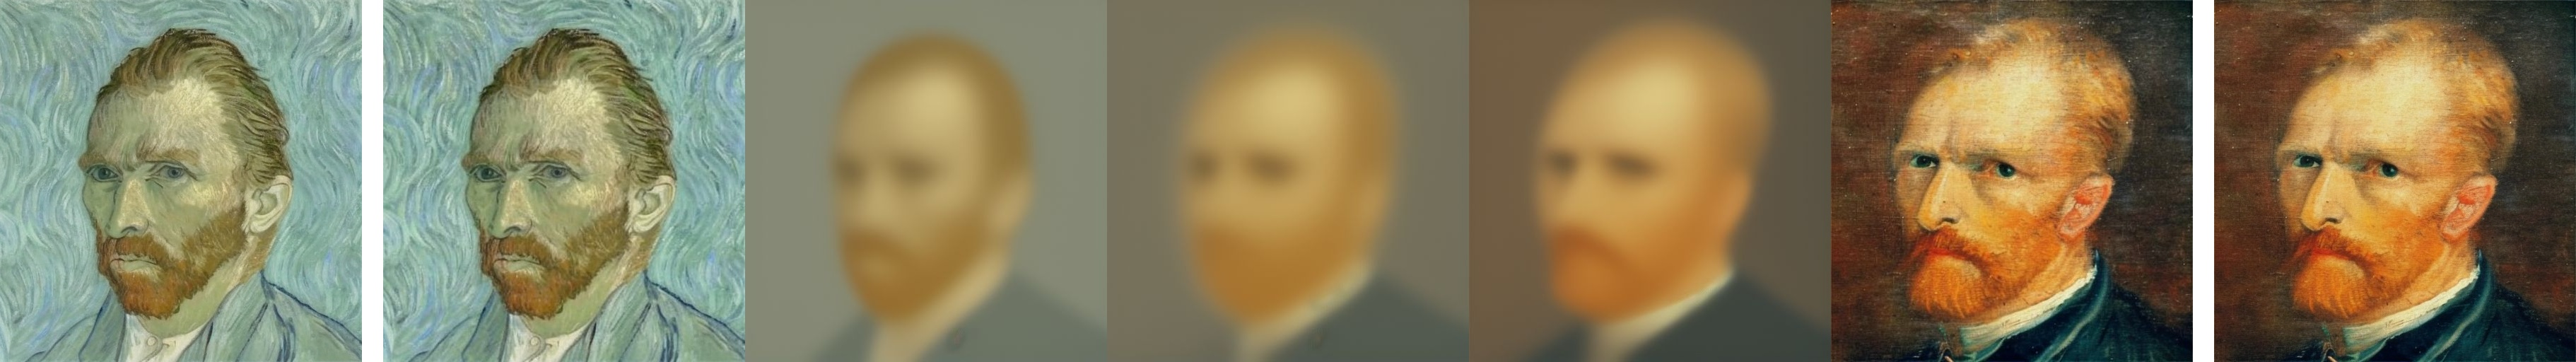
\includegraphics[width=\interpw]{assets/interpolation/image/5/vangogh_lerp.jpg}}      \\ \addlinespace[1.7pt]
        \rotatebox{90}{\hspace{1.5mm}\textcolor{GREEN}{SLERP}}                & {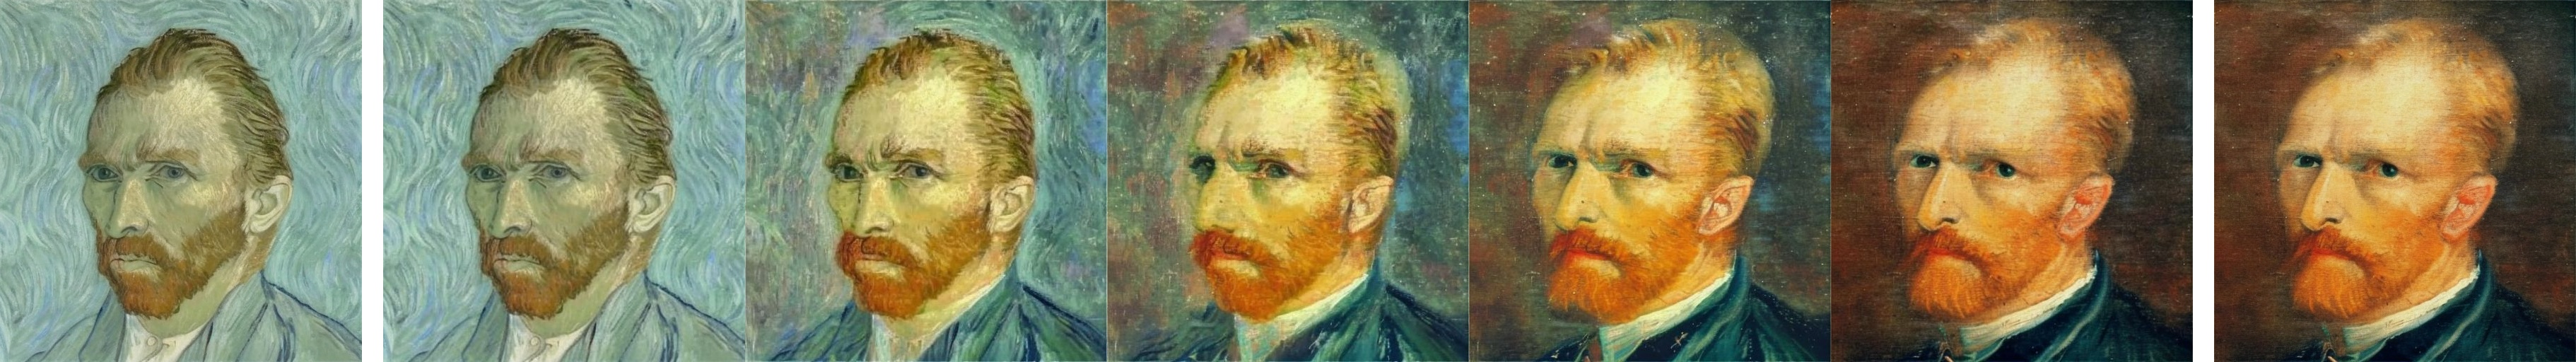
\includegraphics[width=\interpw]{assets/interpolation/image/5/vangogh_slerp.jpg}}     \\ \addlinespace[1.7pt]
        \rotatebox{90}{\hspace{3mm}\textcolor{PURPLE}{NAO}}                   & {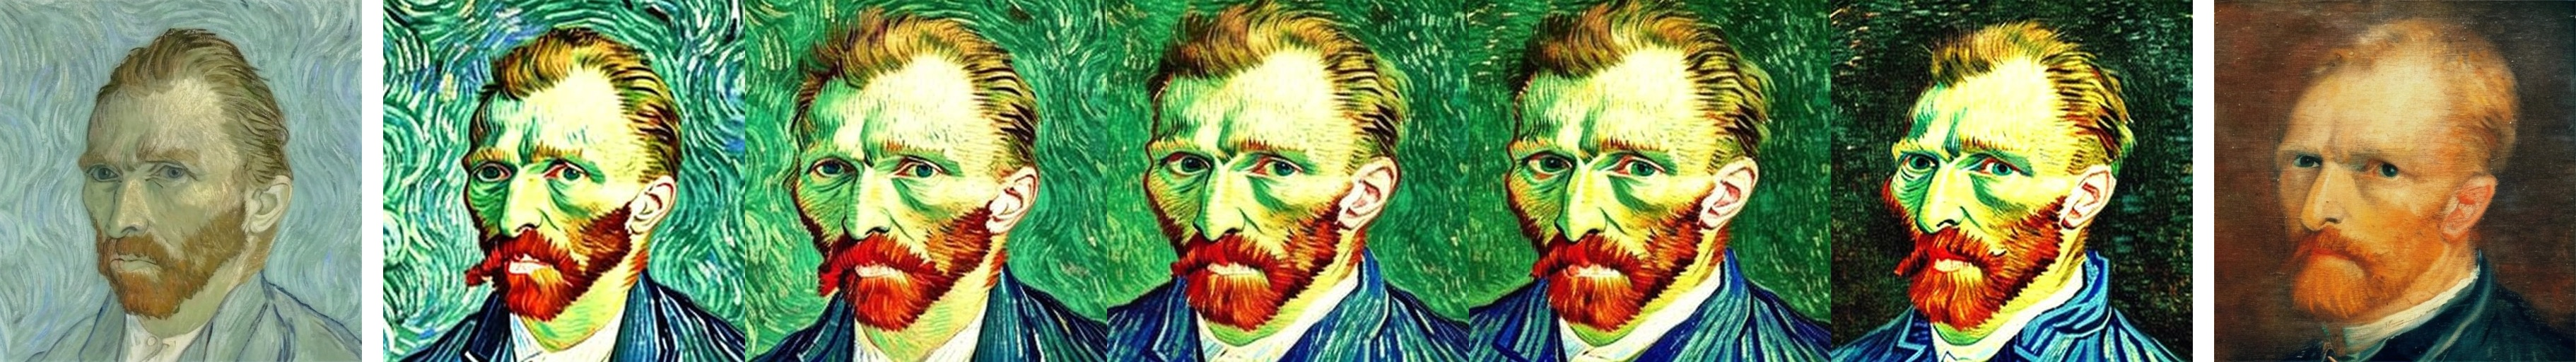
\includegraphics[width=\interpw]{assets/interpolation/image/5/vangogh_nao.jpg}}       \\ \addlinespace[1.7pt]
        \rotatebox{90}{\hspace{0.5mm}\textcolor{PINK}{NoiseDiff}}             & {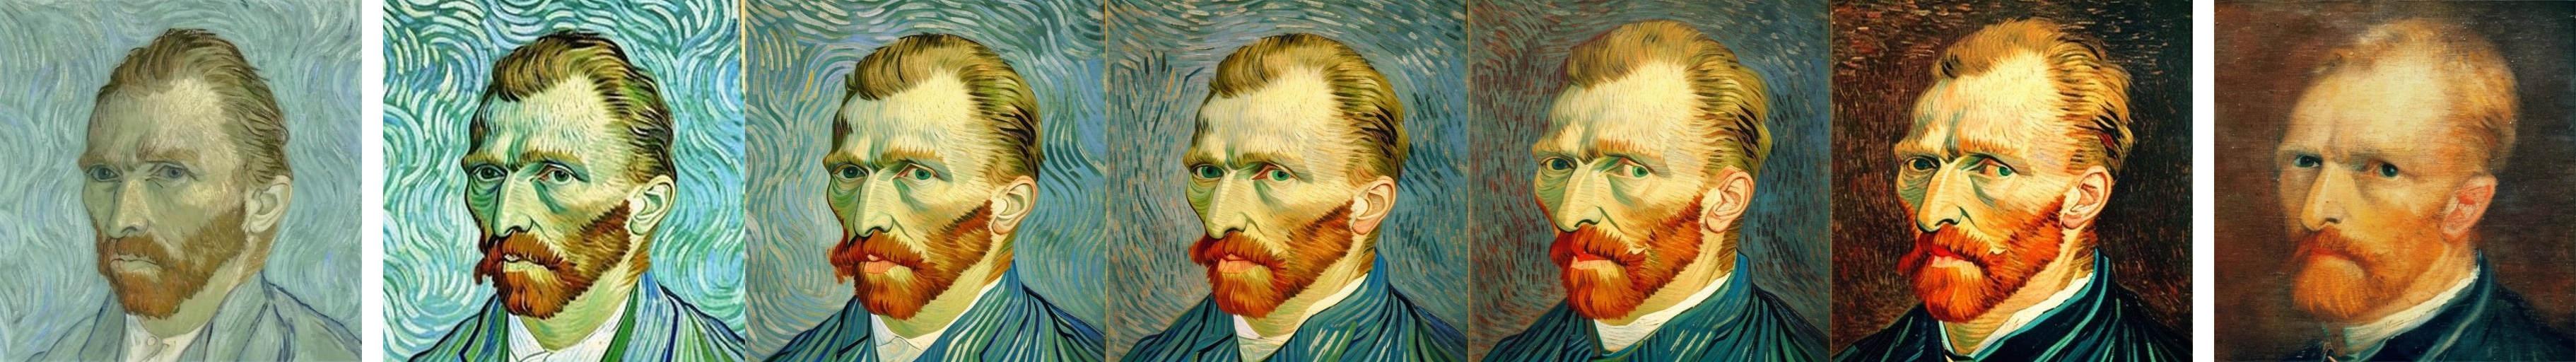
\includegraphics[width=\interpw]{assets/interpolation/image/5/vangogh_noisediff.jpg}} \\ \addlinespace[1.7pt]
        \rotatebox{90}{\hspace{1.5mm}\textcolor{ORANGE}{GeoDiff}}             & {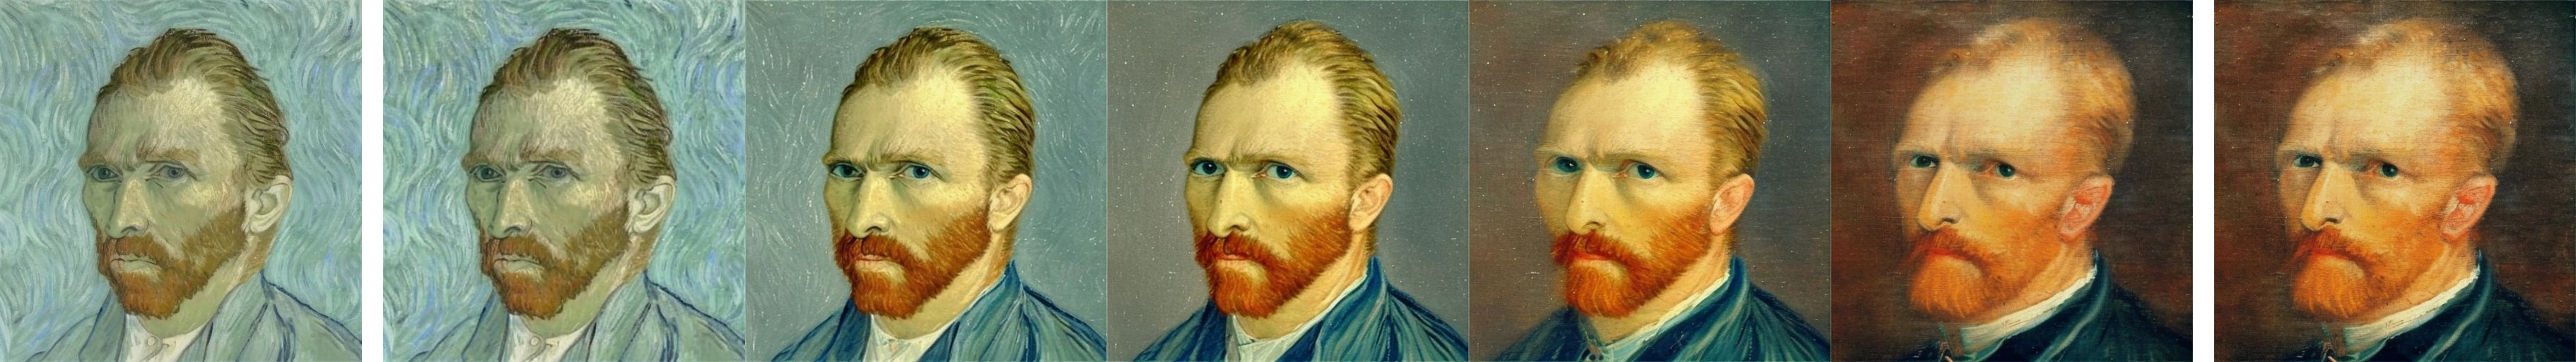
\includegraphics[width=\interpw]{assets/interpolation/image/5/vangogh_geodiff.jpg}}   \\ \addlinespace[1.2pt]
        \rotatebox{90}{\textcolor{GRAY}{FIM\tiny{-based}}}                    & {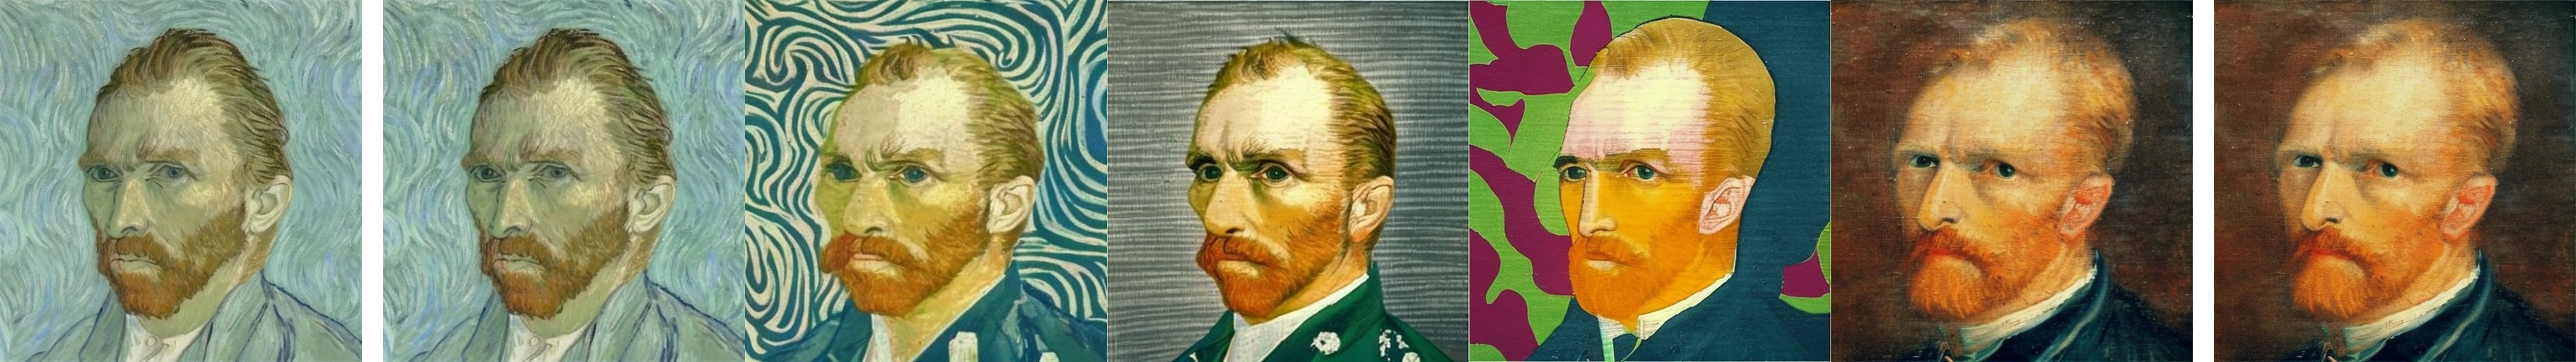
\includegraphics[width=\interpw]{assets/interpolation/image/5/vangogh_fim.jpg}}       \\ \addlinespace[1.9pt]
        \rotatebox{90}{\hspace{3mm}\textcolor{BLACK}{Ours}}                   & {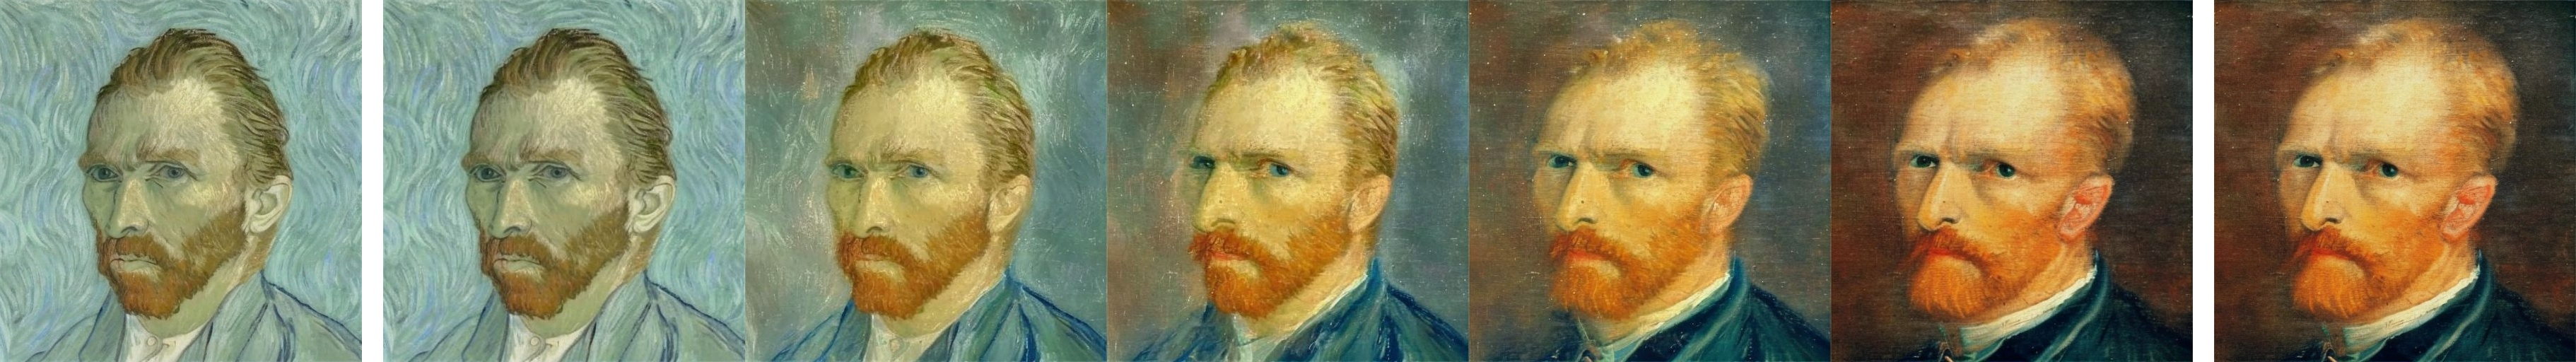
\includegraphics[width=\interpw]{assets/interpolation/image/5/vangogh_ours.jpg}}      \\ \addlinespace[1.7pt]
                                                                              & 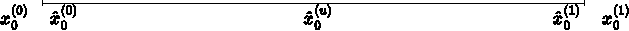
\includegraphics[scale=0.62]{assets/interpolation/imagelabel.drawio-crop.pdf}          \\ \addlinespace[3.0pt]
                                                                              & \scriptsize{MorphBench (metamorphosis)}                                                \\ \addlinespace[6.0pt]
    \end{tabular}
        \caption{
            各手法における補間画像列の定性比較．
            両端は入力画像 $x_0^\sss{0}$, $x_0^\sss{1}$，中間は補間結果 $\{\hat{x}_0^\sss{u}\}$ $(u\in[0,1])$ を示す．
            その他の結果は付録~\ref{appendix:additional_results}を参照．
        }
    \label{fig:results_qualitative}
\end{figure}

% \begin{figure*}[t]
%     \centering
%     \scriptsize
%     \setlength{\tabcolsep}{2pt}
%     \renewcommand{\arraystretch}{0}
%     \newlength{\interpw}
%     \setlength{\interpw}{16cm}
%     \begin{tabular}{rc}
%         \raisebox{2.9mm}{\textcolor{BLUE}{LERP}}      & {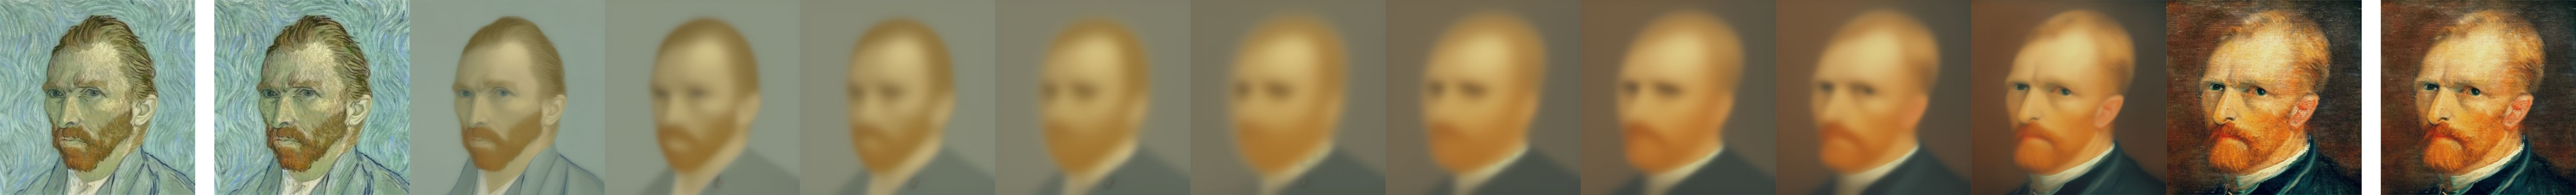
\includegraphics[width=\interpw]{assets/interpolation/image/11/vangogh_lerp.jpg}}      \\ \addlinespace[1.5pt]
%         \raisebox{2.9mm}{\textcolor{GREEN}{SLERP}}    & {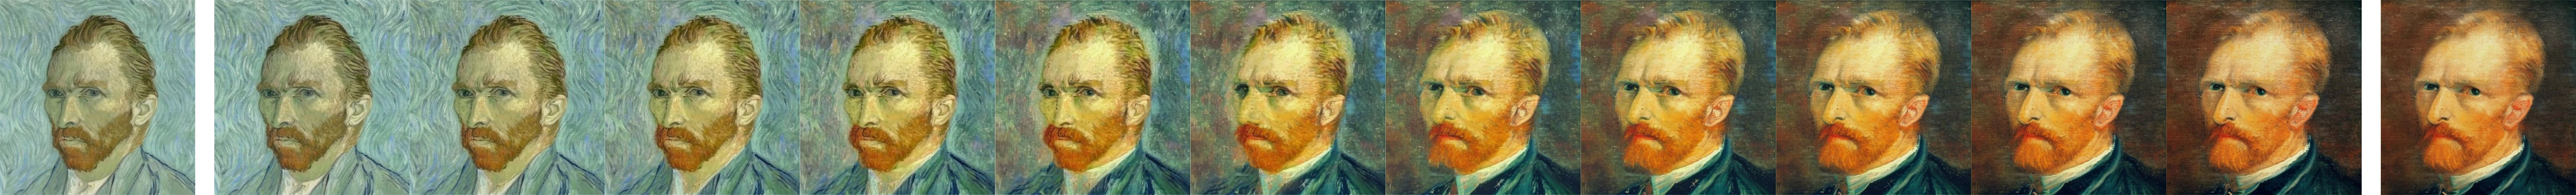
\includegraphics[width=\interpw]{assets/interpolation/image/11/vangogh_slerp.jpg}}     \\ \addlinespace[1.5pt]
%         \raisebox{2.9mm}{\textcolor{PURPLE}{NAO}}     & {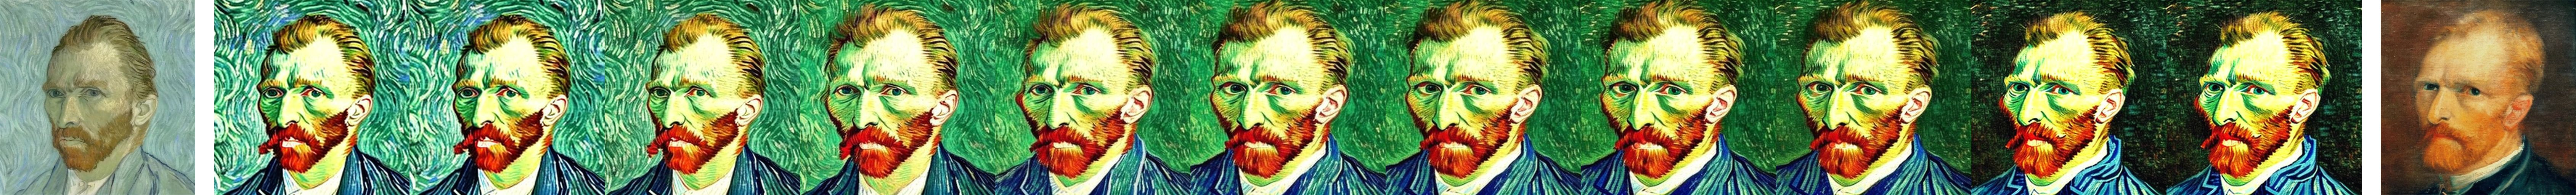
\includegraphics[width=\interpw]{assets/interpolation/image/11/vangogh_nao.jpg}}       \\ \addlinespace[1.5pt]
%         \raisebox{2.9mm}{\textcolor{PINK}{NoiseDiff}} & {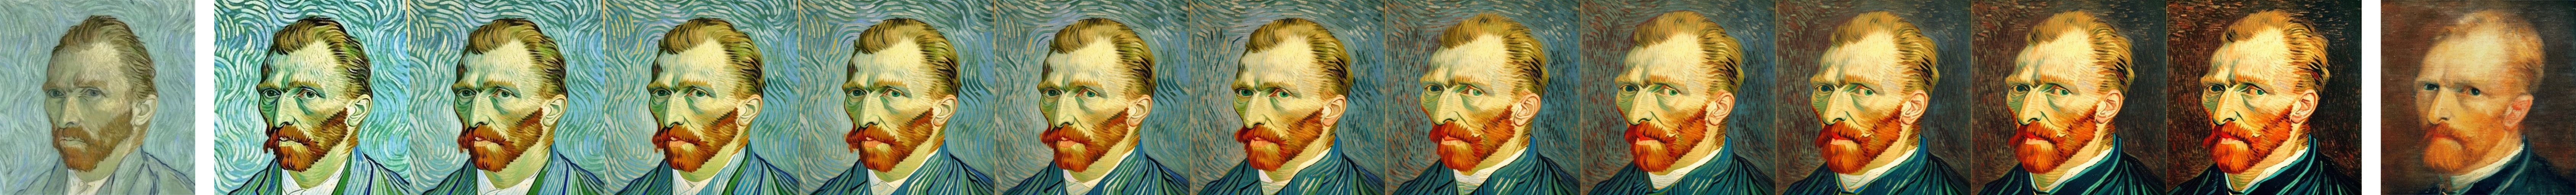
\includegraphics[width=\interpw]{assets/interpolation/image/11/vangogh_noisediff.jpg}} \\ \addlinespace[1.5pt]
%         \raisebox{2.9mm}{\textcolor{ORANGE}{GeoDiff}} & {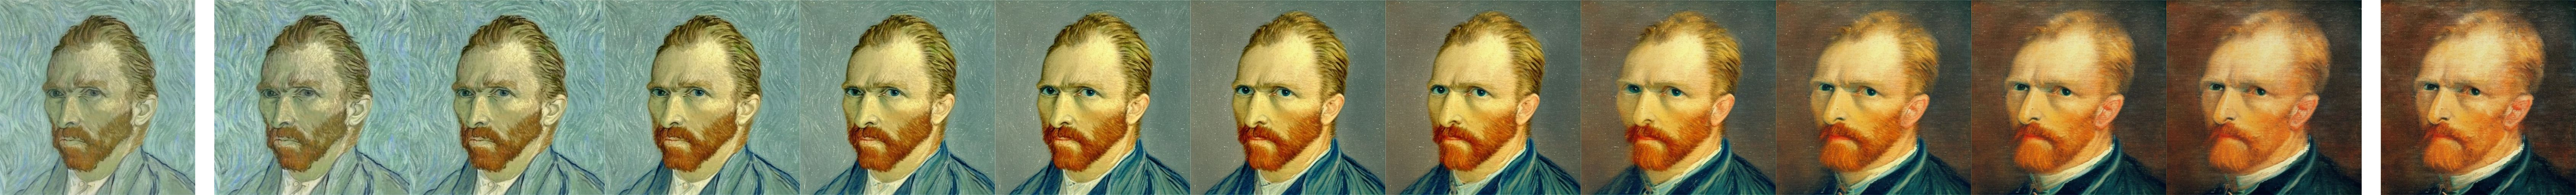
\includegraphics[width=\interpw]{assets/interpolation/image/11/vangogh_geodiff.jpg}}   \\ \addlinespace[1.5pt]
%         \raisebox{2.9mm}{\textcolor{GRAY}{FIM-based}} & {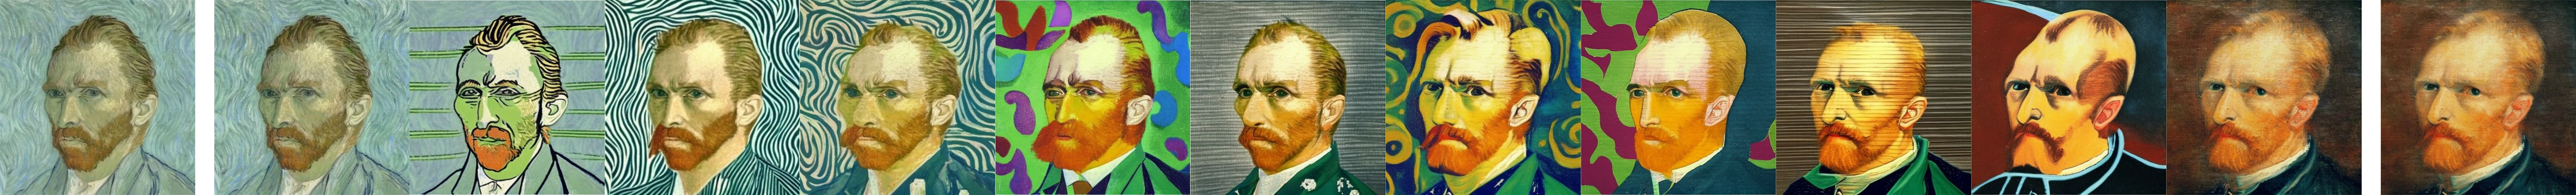
\includegraphics[width=\interpw]{assets/interpolation/image/11/vangogh_fim.jpg}}       \\ \addlinespace[1.5pt]
%         \raisebox{2.9mm}{\textcolor{BLACK}{Ours}}     & {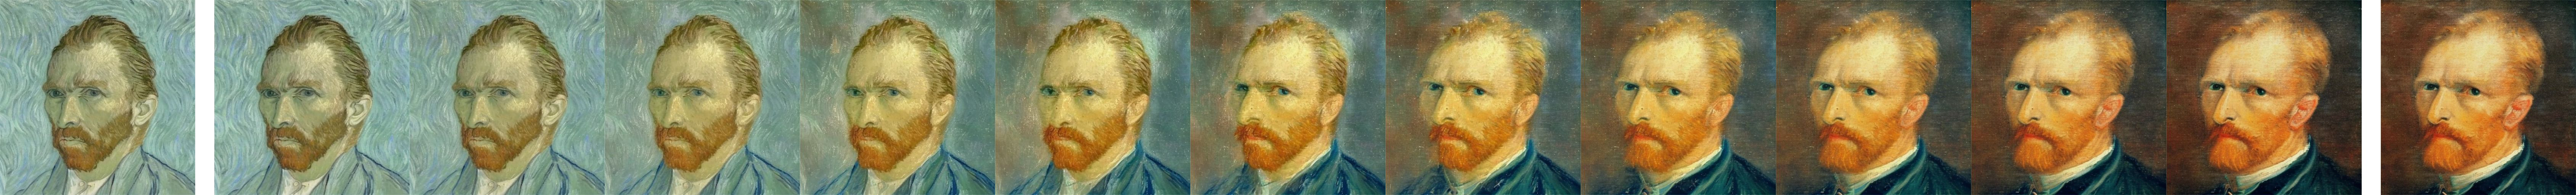
\includegraphics[width=\interpw]{assets/interpolation/image/11/vangogh_ours.jpg}}      \\ \addlinespace[1.5pt]
%                                                       & 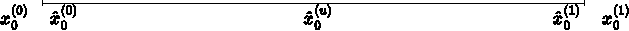
\includegraphics[scale=1.47]{assets/interpolation/imagelabel.drawio-crop.pdf}                  \\ \addlinespace[1.5pt]
%                                                       & MorphBench (metamorphosis)                                                                \\ \addlinespace[6.0pt]
%     \end{tabular}
%     %     \caption{
%     %     Qualitative examples of interpolated image sequences for MB(M) and AF (Dog).
%     %     The images at both ends are the given endpoints $x_0^\sss{0}$ and $x_0^\sss{1}$, and the middle images are the interpolated results $\{\hat{x}_0^\sss{u}\}$ for $u\in[0,1]$.
%     %     See also \cref{fig:results_qualitative_appendix} in \cref{appendix:additional_results}.
%     % }
%     \label{fig:results_qualitative}
% \end{figure*}

\subsection{動画フレーム補間}
\label{sec:video_interp}

前節の間接指標を補完するため，DAVIS~\cite{Perazzi2016}，Pexels Human，RealEstate10K（RE10K）~\cite{Zhou2018} の3ベンチマークで地面真値の中間フレームと MSE・LPIPS を用いて評価した．

% \begin{table}[t]
%     \centering
%     \scriptsize
%     \caption{動画フレーム補間の定量評価結果．}
%     \label{tab:video_results}
%     \setlength{\tabcolsep}{2.85pt}
%     \begin{tabular}{l rrr rrr}
%         \toprule
%          & \multicolumn{3}{c}{MSE $\downarrow$ $(\times10^{-3})$} & \multicolumn{3}{c}{LPIPS $\downarrow$} \\
%         \cmidrule(lr){2-4}\cmidrule(lr){5-7}
%         手法 & DAVIS & Human & RE10K & DAVIS & Human & RE10K \\
%         \midrule
%         LERP      & \underline{12.135} &  4.566 &  6.299 & 0.590 & 0.379 & 0.377 \\
%         SLERP     & 15.440 &  6.080 &  6.128 & 0.487 & 0.320 & 0.301 \\
%         NAO       & 108.211 & 99.867 & 121.680 & 0.679 & 0.668 & 0.664 \\
%         NoiseDiff &  46.881 & 41.994 &  28.867 & 0.561 & 0.552 & 0.482 \\
%         GeoDiff   & 13.253 & \underline{3.363} & \underline{5.941} & \underline{0.334} & \underline{0.184} & \underline{0.229} \\
%         FIM-based & 30.172 & 11.638 & 12.679 & 0.535 & 0.388 & 0.373 \\
%         \midrule
%         \textbf{提案} & \textbf{8.777} & \textbf{2.018} & \textbf{2.771} & \textbf{0.318} & \textbf{0.170} & \textbf{0.178} \\
%         \bottomrule
%     \end{tabular}
% \end{table}

提案手法は全データセットで MSE・LPIPS ともに最低値を達成し，次点手法との改善はすべて統計的有意であった．
定性比較では，GeoDiff は動体補間は成功するが水面の波紋等の細かいテクスチャを平滑化し，提案手法は輪郭・形状・テクスチャを最も忠実に再現することを，地面真値との比較により確認した．

\subsection{ガイダンス補正による生成}
\label{sec:guidance}

\subsubsection{実験設定．}
Stable Diffusion v2.1-base~\cite{Rombach2022}（$T=50$）を用い，MS-COCO 2014 検証セット~\cite{Lin2014} のテキストプロンプトから3万枚を生成して，FID~\cite{Martin2017} と CLIP Score~\cite{Radford2021} で評価した．
比較手法は CFG~\cite{Ho2021} および CFG++~\cite{Chung2025} である．

\begin{table*}[t]
    \centering
    \footnotesize
    \caption{ガイダンス補正（左）および蒸留（右）の定量評価結果．}
    \label{tab:guidance_results}
    \begin{minipage}{0.65\textwidth}
        \centering
        \setlength{\tabcolsep}{6pt}
        \begin{tabular}{l cccccc}
            \toprule
             & \multicolumn{2}{c}{$w=5.0$} & \multicolumn{2}{c}{$w=7.5$} & \multicolumn{2}{c}{$w=12.5$} \\
            \cmidrule(lr){2-3}\cmidrule(lr){4-5}\cmidrule(lr){6-7}
             & FID $\downarrow$ & CLIP $\uparrow$ & FID $\downarrow$ & CLIP $\uparrow$ & FID $\downarrow$ & CLIP $\uparrow$ \\
            \midrule
            CFG     & \underline{11.69} & 0.313 & 14.29 & 0.314 & \underline{17.28} & 0.315 \\
            CFG++   & 11.87 & 0.313 & \underline{13.98} & 0.314 & 17.76 & 0.315 \\
            \midrule
            \textbf{提案} & \textbf{11.53} & 0.313 & \textbf{13.81} & 0.314 & \textbf{16.04} & 0.315 \\
            \bottomrule
        \end{tabular}
    \end{minipage}
    \hfill
    \begin{minipage}{0.30\textwidth}
        \centering
        \setlength{\tabcolsep}{6pt}
        \begin{tabular}{l cc}
            \toprule
             & FID $\downarrow$ & CLIP $\uparrow$ \\
            \midrule
            CFG  & 17.91 & 0.306 \\
            \textbf{提案} & \textbf{16.98} & 0.306 \\
            \bottomrule
        \end{tabular}
    \end{minipage}
\end{table*}


\begin{figure}[t]
    \centering
    \fontsize{6}{7.2}\selectfont
    \setlength{\tabcolsep}{1.0pt}
    \renewcommand{\arraystretch}{0}
    \newlength{\guidimgw}
    \setlength{\guidimgw}{1.54cm}
    \begin{tabular}{r ccccc}
        % Row 1: CFG
        \rotatebox{90}{\hspace{6.6mm}CFG}
        & 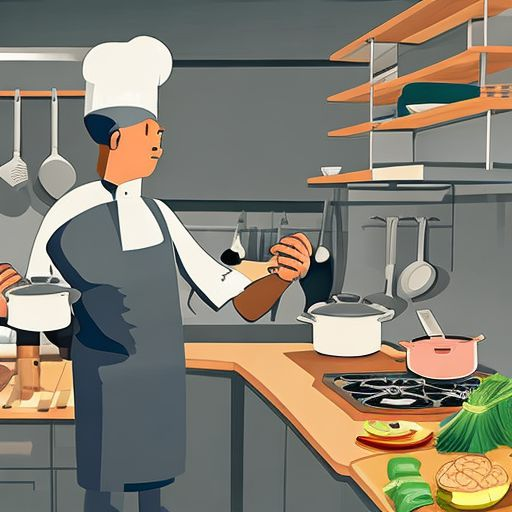
\includegraphics[width=\guidimgw]{assets/guidance/146961_cfg.jpg}
        & 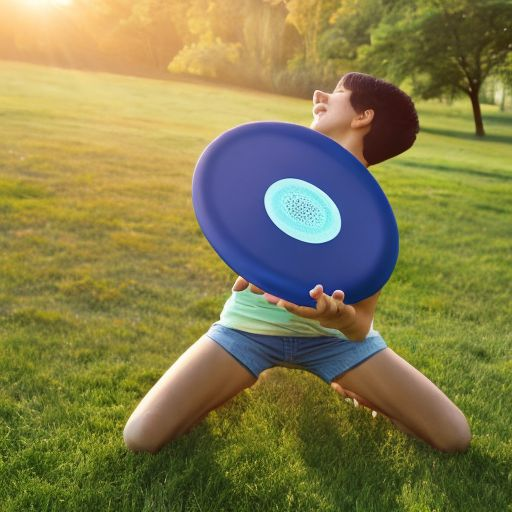
\includegraphics[width=\guidimgw]{assets/guidance/146190_cfg.jpg}
        & 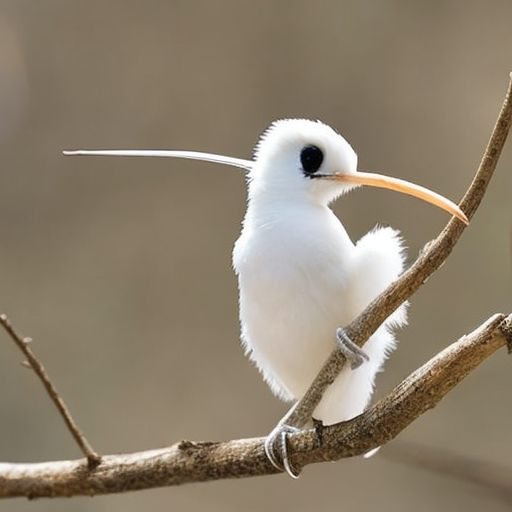
\includegraphics[width=\guidimgw]{assets/guidance/122838_cfg.jpg}
        & 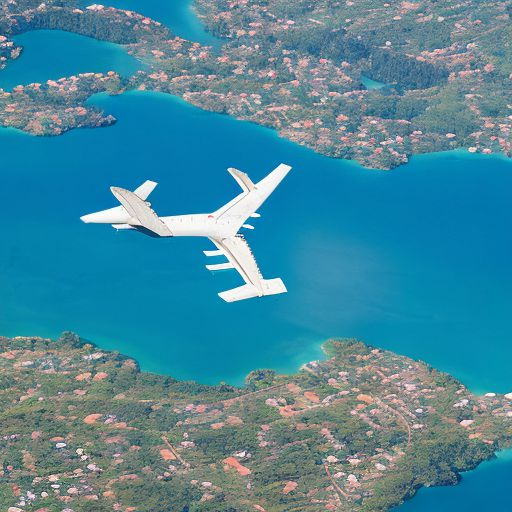
\includegraphics[width=\guidimgw]{assets/guidance/0472_cfg.jpg}
        & 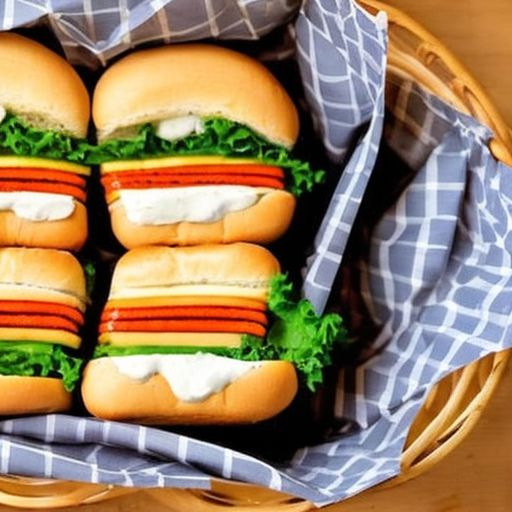
\includegraphics[width=\guidimgw]{assets/guidance/80690_cfg.jpg}
        \\ \addlinespace[1.2pt]
        % Row 2: CFG++
        \rotatebox{90}{\hspace{3mm}CFG++}
        & 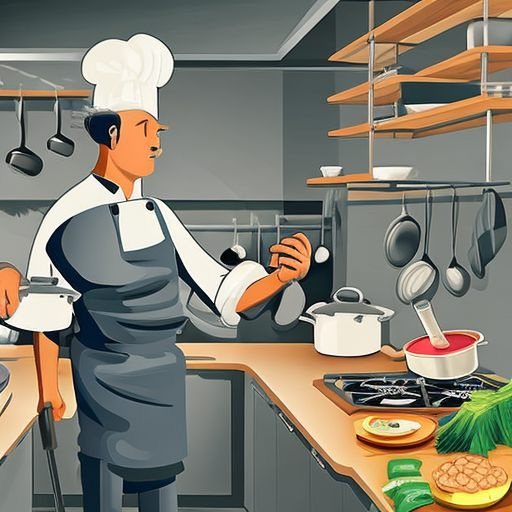
\includegraphics[width=\guidimgw]{assets/guidance/146961_cfgpp.jpg}
        & 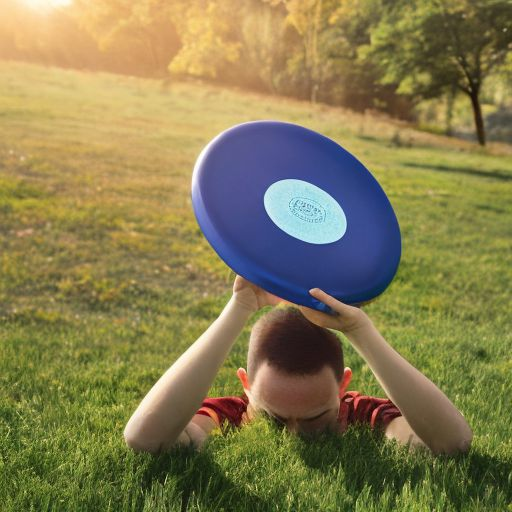
\includegraphics[width=\guidimgw]{assets/guidance/146190_cfgpp.jpg}
        & 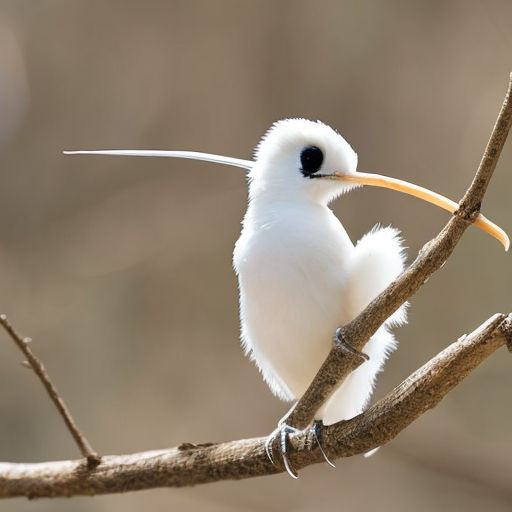
\includegraphics[width=\guidimgw]{assets/guidance/122838_cfgpp.jpg}
        & 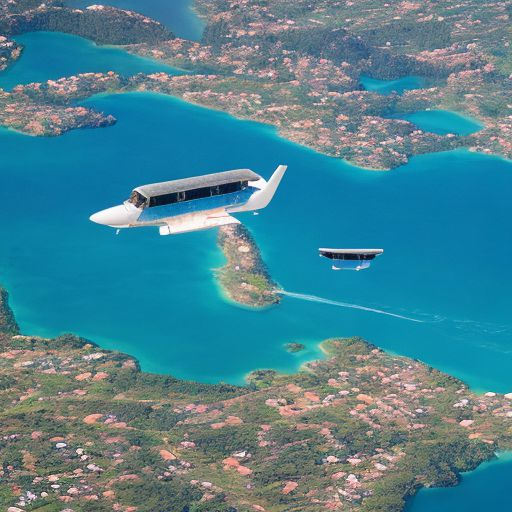
\includegraphics[width=\guidimgw]{assets/guidance/0472_cfgpp.jpg}
        & 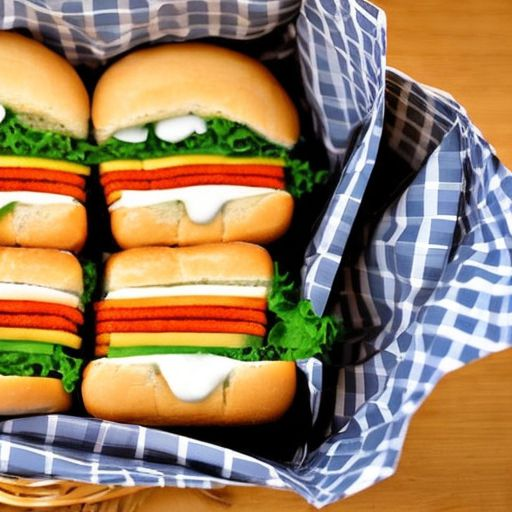
\includegraphics[width=\guidimgw]{assets/guidance/80690_cfgpp.jpg}
        \\ \addlinespace[1.2pt]
        % Row 3: Ours
        \rotatebox{90}{\hspace{6.5mm}Ours}
        & 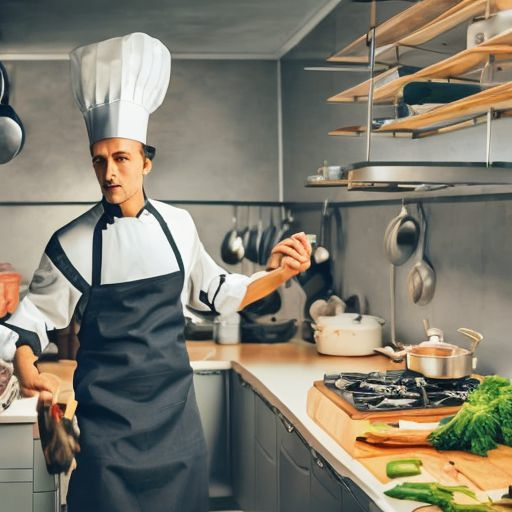
\includegraphics[width=\guidimgw]{assets/guidance/146961_ours.jpg}
        & 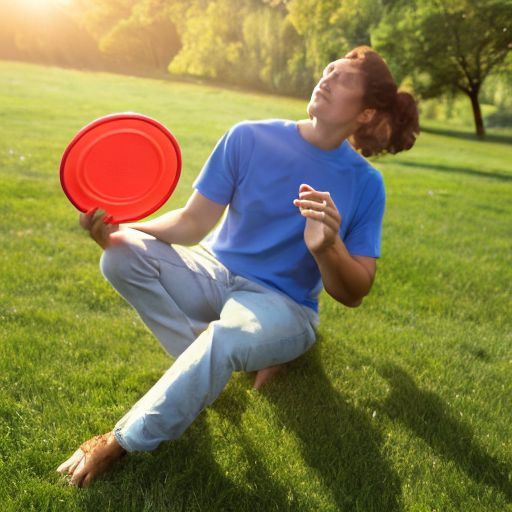
\includegraphics[width=\guidimgw]{assets/guidance/146190_ours.jpg}
        & 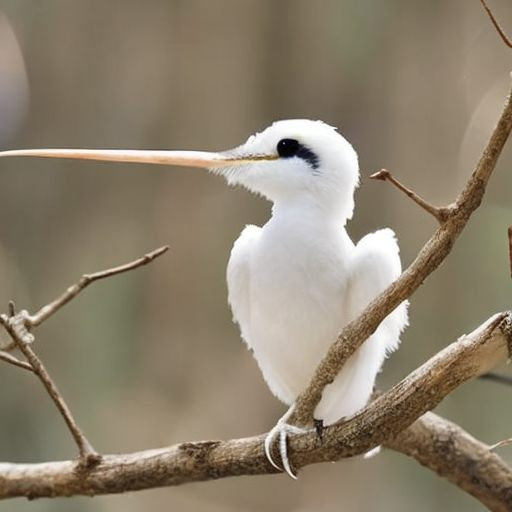
\includegraphics[width=\guidimgw]{assets/guidance/122838_ours.jpg}
        & 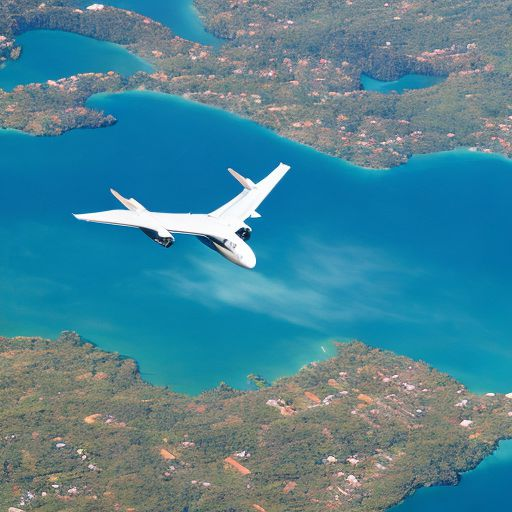
\includegraphics[width=\guidimgw]{assets/guidance/0472_ours.jpg}
        & 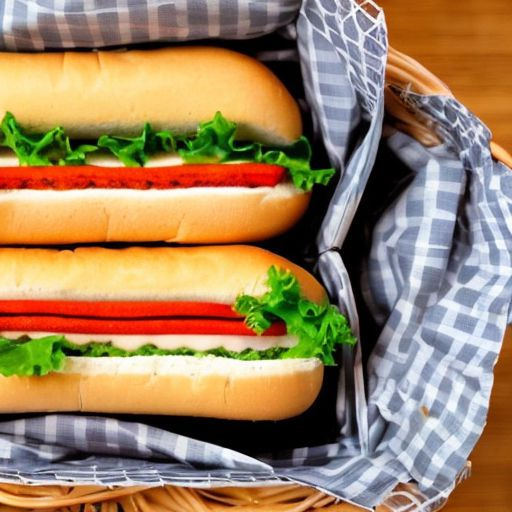
\includegraphics[width=\guidimgw]{assets/guidance/80690_ours.jpg}
        \\ \addlinespace[2.5pt]
        % Prompts
         & \parbox{0.9\guidimgw}{\centering ``A man is cooking in a crowded kitchen''}
         & \parbox{0.9\guidimgw}{\centering ``A person is in the grass holding a frisbee''}
         & \parbox{0.9\guidimgw}{\centering ``A small white bird with a long beak on a branch''}
         & \parbox{0.9\guidimgw}{\centering ``A plane flies over water with two islands nearby''}
         & \parbox{0.9\guidimgw}{\centering ``A couple of sub sandwiches are in basket''}
        \\
    \end{tabular}
    \caption{
        Qualitative comparison between CFG, CFG++, and Ours
    }
    \label{fig:guidance_qualitative}
\end{figure}

\subsubsection{結果．}
\Cref{tab:guidance_results} に示すように，提案手法はすべての CFG スケール $w$ でFIDを一貫して改善し，CLIPスコアは維持した．
CFG++ はFIDの改善が安定せず，ハイパーパラメータへの感度が示唆される．
提案ガイダンス補正はガイダンス項のみを修正するため，蒸留時（LCM~\cite{Luo2023}）に適用することで，4ステップ推論においても FID を 17.91 から 16.98 に改善し，推論コストを増やさずに品質向上を学生モデルに継承できることを確認した（5試行すべてで改善，$p < 0.05$）．

\section{結論}

本稿では，スコア関数のヤコビアンから導かれる，拡散モデルのノイズ空間上におけるリーマン計量を提案した．
提案計量は，ヤコビアンのスペクトル構造を通じてデータ多様体の接線・法線を分離し，追加学習なしに任意の事前学習済みモデルから計算できる．
実験では，画像・動画の複数ベンチマークにおいて提案測地線が全指標で先行手法を上回り，また接線・法線分解による CFG 補正が CLIPスコアを維持しつつ FID を改善することを確認した．
蒸留モデルにも適用可能であり，4ステップの高速推論でも品質の向上を確認した．
今後の展望として，ノイズ空間における意味的編集やフローマッチングへの拡張，ヤコビアンの計算コスト削減による高速化が課題である．
\clearpage

\bibliographystyle{miru2026j}
\bibliography{main}

\clearpage

\appendix

\section{予備知識}
\label{sec:preliminaries}

\subsection{リーマン幾何}
\label{appendix:riemannian_geometry}

\subsection{拡散モデル}
\label{appendix:diffusion_models}

\section{命題の詳細}
\label{appendix:proposition}

\section{比較手法の詳細}
\label{appendix:comparison}

\subsection{各比較手法}
\label{appendix:comparison_methods}

\subsection{補間手法の計算コスト}
\label{appendix:comp_cost}

\subsection{プロンプト調整}
\label{appendix:prompt_adjustment}

\section{実験設定の詳細}
\label{appendix:experimental}

\subsection{合成2Dデータセット}
\label{appendix:synthetic}

\subsection{画像補間データセット}
\label{appendix:image_interpolation_datasets}

\subsection{蒸留のハイパーパラメータ}
\label{appendix:hyperparameters}

\section{追加実験結果}
\label{appendix:additional_results}

\subsection{アブレーション研究}
\label{appendix:ablation}

\end{document}
